\documentclass[
oneside,numbers=noenddot,headinclude,
footinclude=true,cleardoublepage=empty,
dottedtoc,paper=a4,fontsize=12pt,
]{scrreprt}
\usepackage{graphicx}
\usepackage[french]{babel}
\usepackage[utf8]{inputenc}
\usepackage[french]{babel}
\usepackage[T1]{fontenc}
\usepackage{classicthesis}
\usepackage{csquotes}
\usepackage{acronym}
\usepackage{booktabs}
\usepackage{subfiles}
\usepackage[a4paper,left=3cm, right=3cm, top=3.00cm, bottom=3.00cm]{geometry}
\usepackage{scrlayer-scrpage}
\KOMAoptions{singlespacing=true}
% \usepackage[oldstylenums]{kpfonts}
% \usepackage[osf]{libertine}
%\usepackage[light,condensed,math]{iwona}
\renewcommand{\sfdefault}{iwona}
% \usepackage{lmodern}
% \usepackage{cfr-lm}
% \usepackage[urw-garamond]{mathdesign}
% \usepackage[default,osfigures]{opensans}
%\usepackage[sfdefault]{FiraSans}


\graphicspath{{gfx/}}
\linespread{1.3}
\titleformat{\chapter}[display]
{\relax}{\vspace*{-3\baselineskip}\makebox[\linewidth][r]{\color{halfgray}\chapterNumber\thechapter}}{0pt}%
{\raggedright\spacedallcaps}[\normalsize\vspace*{.8\baselineskip}\titlerule]

\usepackage[T1]{fontenc}
\usepackage{hyperref}
\usepackage{titlesec}
\usepackage{longtable}
\usepackage{xcolor}
%\usepackage{biblatex}
 
\usepackage{hyperref}
\hypersetup{
	colorlinks=true,  
	linkcolor=blue,  
	urlcolor=blue, 
	filecolor=magenta,  
	citecolor=blue,
	pdfborder={56 0 0}  
}
\begin{document}
\documentclass{report}
\usepackage{graphicx}
\usepackage[french]{babel}
\usepackage[T1]{fontenc}
 
\begin{document}
	\author{Tshibangu Ntumba Kenny}
	
	\begin{titlepage}
		
		\centering
		
		\textbf{\Large RÉPUBLIQUE DÉMOCRATIQUE DU CONGO
			MINISTÈRE DE L’ENSEIGNEMENT SUPÉRIEUR ET UNIVERSITAIRE}
		\vspace{1.5cm}
		 
		 
\includegraphics[width=0.5\textwidth]{Logo.jpg}
		 \vspace{3.5cm}
		 
		 
		 \textbf{\Large "  MISE EN PLACE D'UN SYSTÈME DE SECURITE DANS UN SERVEUR WEB "}
		 \vspace{2.5cm}
		 
		  \large Par :\textbf{Tshibangu Ntumba Kenny} 
		  
		  \paragraph{ } Travail de fin d’études présenté en vue de l’obtention
		  du grade de licencié en Sciences Informatiques
		\paragraph{ } \Large{ Option : Réseau et Infrastructure}
		 \vfill
		 {\LARGE Année Académique 2022-2023}
	\end{titlepage}
\begin{center}
\tableofcontents
\pagebreak
\end{center}
	    
	\begin{Huge}
	Introduction Générale
	\end{Huge}
	 
 \section{ Quelques petites Définition}
 \subsection{La Securite Informatique }
 
 
 \paragraph{ }  La sécurité informatique est l'ensemble des mesures techniques, organisationnelles et juridiques mises en place pour protéger les systèmes informatiques, les réseaux et les données contre les attaques, les pertes ou les altérations. Elle vise à garantir la confidentialité, l'intégrité et la disponibilité des informations stockées sur les systèmes informatiques, ainsi que la protection de la vie privée et des droits de propriété intellectuelle.  
 
 \paragraph{ } La sécurité informatique englobe un large éventail de domaines, tels que la sécurité des réseaux, la sécurité des systèmes d'exploitation, la sécurité des applications, la sécurité des données, la sécurité physique, la gestion des identités et des accès, la conformité aux normes de sécurité, la surveillance et la détection des incidents de sécurité, ainsi que la réponse aux incidents de sécurité.
 
 \paragraph{ }  La sécurité informatique est devenue un enjeu majeur dans le monde numérique d’aujourd’hui, où les attaques informatiques sont de plus en plus sophistiquées et fréquentes. La mise en place d'une politique de sécurité informatique efficace est donc essentielle pour protéger les systèmes informatiques et les données sensibles contre les menaces potentielles et assurer la continuité des activités des organisations qui les utilisent.
 \pagebreak
  
 \hbox{\includegraphics[width=0.5\textwidth]{image_sec.png}}
  \paragraph{ }
 \hbox{ La sécurité informatique englobe plusieurs domaines d'applications :}
 \vspace{5mm}
   \textendash \space   sécurité physique et environnementale ;
  \paragraph{ }
   \textendash \space   sécurité de l’exploitation ;
  \paragraph{ }
   \textendash \space  sécurité des réseaux ;
 \paragraph{ }
   \textendash \space  sécurité logique, sécurité applicative et sécurité de l’information ;
   
   \paragraph{ }
   \textendash \space cybersécurité.
   
  \subsection{ La Cyber Sécurité }
  \paragraph{ }
  La cybersécurité, également appelée sécurité informatique ou sécurité des technologies de l'information, est l'ensemble des mesures techniques, organisationnelles et juridiques mises en place pour protéger les systèmes informatiques, les réseaux et les données contre les attaques, les pertes ou les altérations. Elle vise à garantir la confidentialité, l'intégrité et la disponibilité des informations stockées sur les systèmes informatiques, ainsi que la protection de la vie privée et des droits de propriété intellectuelle.
  \paragraph{ }
  La cybersécurité concerne la sécurité informatique et des réseaux des environne-
ments connectés à Internet et accessibles via le cyberespace. Elle peut être mise en
défaut, entre autres, par des cyberattaques informatiques. Du fait de l’usage extensif
d’Internet, de nouvelles menaces sont apparues générant des risques additionnels
dont les impacts, de niveaux d’importance variables, peuvent affecter les individus,
les organisations ou les États. 
   \paragraph{ }
  La cybersécurité est devenue un enjeu majeur dans le monde numérique d'aujourd'hui, où les attaques informatiques sont de plus en plus sophistiquées et fréquentes. Elle est essentielle pour protéger les systèmes informatiques et les données sensibles contre les menaces potentielles et assurer la continuité des activités des organisations qui les utilisent. La cybersécurité est également importante pour protéger les utilisateurs finaux, tels que les consommateurs et les employés, contre les risques de vol d'identité, de fraude en ligne et d'autres formes de cybercriminalité.
  \paragraph{ }
  Les points essentiels englobés par la cybersécurité comprennent :
  \space \paragraph{ }


\paragraph{1. La confidentialité :}\paragraph{} la protection des données contre les accès non autorisés. Cela inclut la protection des données personnelles, des secrets commerciaux, des informations financières et autres informations sensibles.

\paragraph{2. L'intégrité :}\paragraph{} la protection des données contre les altérations non autorisées. Cela inclut la garantie que les données sont exactes et fiables.

\paragraph{3. La disponibilité :} \paragraph{}la garantie que les systèmes, les réseaux et les données sont accessibles et fonctionnent correctement, et que les interruptions de service sont minimisées.

\paragraph{4. L'authenticité:}  \paragraph{}la garantie que les utilisateurs sont bien ceux qu'ils prétendent être, et que les données sont bien celles qu'elles prétendent être.

\paragraph{5. La non-répudiation: } \paragraph{}la garantie qu'une personne ne peut pas nier avoir effectué une action ou avoir envoyé des données.

\paragraph{6. La résilience :} \paragraph{}la capacité des systèmes et des réseaux à résister aux attaques et à récupérer rapidement en cas d'incident.
\pagebreak

\paragraph{7. La conformité :} \paragraph{}le respect des lois, des réglementations et des normes en matière de sécurité informatique.

\paragraph{8. La sensibilisation :}\paragraph{} l'éducation et la formation des utilisateurs pour qu'ils comprennent les risques liés à la sécurité informatique et les meilleures pratiques à suivre pour les éviter.

Ces points essentiels sont interconnectés et doivent être pris en compte dans toute stratégie de cybersécurité efficace.
  \subsection {Quelques mots sur  les Serveurs }
  \vspace{4mm}
  \paragraph{ \includegraphics[width=0.5\textwidth]{salle-serveur.jpg}}
  \paragraph{ }
  Les serveurs sont des ordinateurs ou des systèmes informatiques qui fournissent des services ou des ressources à d'autres ordinateurs ou utilisateurs sur un réseau. Ils peuvent être utilisés pour stocker des données, héberger des sites Web, exécuter des applications et bien plus encore. Il existe différents types de serveurs, tels que les serveurs de fichiers, les serveurs de messagerie, les serveurs de bases de données et les serveurs de jeux en ligne. Les serveurs sont souvent utilisés pour fournir des services à distance, ce qui permet aux utilisateurs d'y accéder à partir de n'importe où dans le monde.
  \pagebreak
  \subsection{Les Serveurs Web}
  \vspace{4mm}
  \paragraph{
  \includegraphics[width=0.5\textwidth]{Server_web.png}}
  \paragraph{ }
  Les serveurs Web sont des ordinateurs ou des programmes informatiques qui fournissent des pages Web aux clients qui les demandent via un navigateur Web. Ils sont utilisés pour héberger des sites Web et distribuer du contenu en ligne. Les serveurs Web peuvent exécuter différents types de logiciels, tels que Apache, Nginx, Microsoft IIS et bien d'autres. Les pages Web sont généralement créées en utilisant des langages de programmation Web tels que HTML, CSS et JavaScript. Les serveurs Web peuvent également exécuter des applications Web, telles que des forums en ligne, des blogs, des magasins en ligne et bien plus encore.
   
  \subsection{Quelques vulnérabilités Sur Les Serveurs Web }
  \paragraph{ }
  Il y a plusieurs vulnérabilités qui peuvent affecter un serveur web, en voici quelques exemples :
  \paragraph{ }
  $\bullet$ Injection SQL : Cette vulnérabilité permet à un attaquant d'injecter du code SQL malveillant dans une requête pour détourner le contrôle de la base de données.
  \paragraph{ }
  $\bullet$ Cross-site scripting (XSS) : Cette vulnérabilité permet à un attaquant d'injecter du code malveillant dans une page Web pour voler des informations d'authentification ou d'autres données sensibles.
  \paragraph{ }
  $\bullet$ Vulnérabilités du serveur HTTP : Les serveurs HTTP tels que Apache, Nginx et IIS peuvent être vulnérables à des attaques telles que les dénis de service (DoS) et les dénis de service distribués (DDoS).
  \paragraph{ }
  $\bullet$ Mauvaise configuration : Une mauvaise configuration du serveur web peut permettre aux attaquants d'accéder aux fichiers sensibles ou d'exécuter du code malveillant.
  \paragraph{ }
  $\bullet$ Vulnérabilités du CMS : Les systèmes de gestion de contenu tels que WordPress et Drupal peuvent être vulnérables à des attaques telles que les injections SQL et les attaques de force brute.
  
  
   \section{Contexte de recherche }
   \paragraph{ } Ce travail s'appuie sur les différents domaines   de la  Cybersécurité qui actuellement est déjà devenu un  des points  plus   important dans le domaine de l'informatique 
   Une Solution simple et pratique peut être proposée  \space;
   Pour rendre le serveur Plus sur et plus sécurisé
   \section{Solution technique} 
   \paragraph{ }
   La solution la plus proche et la moins vorace en ressource serait de mettre en place un système de securite qui respecte le nécessaire des normes de securites dans un serveur web actuel.
   \section{Problématique }
   \paragraph{ }
   Sur un Serveur web il existe plusieurs sortes de vulnérabilités par lesquels on peut facilement y accéder Comme : 
     \paragraph {$\bullet$L'injection SQL : }
      en bref c'est une attaque qui consiste a insérer du code SQL malveillant  dans les entrées   d'un formulaires ...
   
   \paragraph{$\bullet$ Cross-Site Scripting(XSS) :} Comme son nom l'indique c'est une faille de securite qui permet un attaquant d'injecter du code malveillant dans une page web ou de faire une redirection vers un site frauduleux 
   \paragraph{ }
   Et j'en passe ;
   \pagebreak
   \paragraph{ }
   Voici les  quelques questions que nous allons nous poser tout au long de ce travail :
   \paragraph{ }
   \textendash \space Quel est le descriptif d'un bon système de securite ?
   \paragraph{ }
   \textendash \space Quels sont les systèmes de securites  que nous allons utiliser ?
   \paragraph{ }
   \textendash \space Sur quel type de serveur web ce système sera efficace ?
   \section{Méthodologie}
   \paragraph{ }
   Pour arriver a une solution plausible  nous allons utiliser une procédure  qui va nous permettre d'installer des machines virtuelles ; différentes machines virtuelles configurée de différentes façon  ;  et tester différentes approches de sécurisation de serveurs et même essayer de les combinées pour voir si le résultat est solide .
  \section{ Techniques }
  \paragraph{ }
  Pour ce travail la technique appropriée sera :
  \subsection{ La Recherche sur Internet :}
  \paragraph{ }
  Parcourir les différents  sites et forums qui proposent des travaux similaires aux miens , des vidéos et tutoriels pour les différentes configurations a faire  pour ce travail ...
    \subsection{La Recherche Documentaire :}
    \paragraph{ }
    Utiliser les différents livres,revues ,archives ;
    Qui , en les utilisant pourront m'aider a atteindre mon but , ma solution solide .
  \subsection{ La Recherche Expérimentale :}
  \paragraph{ }
  Faire des petites expérimentation sur mes machines virtuelles configurées comme des serveurs web  
  \section{Limitation}
  Dans ce travail nous allons nous limiter a utiliser :
  \paragraph{ } (En fonction de l’évolution de mon travail ce point va se remplir ).
  \section{Objectif}
  
  \paragraph{ }L'objectif visé  dans ce travail est de pouvoir mettre en place un système de securite capable de remplir le travail nécessaire qui est actuellement demandé  sur les serveurs web ;
  \paragraph{ } De configurer un serveur web assez performant pour remplir les prérequis    nécessaire qui sont demandés par la communauté  des développeurs   Web qui sont majoritairement amenés a utiliser les Serveurs Web Pour héberger leurs sites internet  .
  
   \chapter{Prochain Chapitre}
    
\end{document} 
 
 
  \chapter{ Les Serveurs}
 \section{Définitions} 
	\begin{figure}[h]
		 \begin{center}
		  \includegraphics[width=0.7\textwidth]{PhotoMemoire/salle-serveur.jpg}
		\caption{Une Salle Serveur \cite{7}}
	\end{center}
	\end{figure}
Les serveurs sont des ordinateurs ou des systèmes informatiques qui fournissent des services ou des ressources à d'autres ordinateurs ou utilisateurs sur un réseau. Ils peuvent être utilisés pour stocker des données, héberger des sites Web, exécuter des applications et bien plus encore. Il existe différents types de serveurs, tels que les serveurs de fichiers, les serveurs de messagerie, les serveurs de bases de données et les serveurs de jeux en ligne. Les serveurs sont souvent utilisés pour fournir des services à distance, ce qui permet aux utilisateurs d'y accéder à partir de n'importe où dans le monde.
 \subsection*{Fonctionnement}
 Le serveur fonctionne en réseau; Peu importe sa mission, il a pour fonction d’écouter les requêtes formulées par les ordinateurs clients et de les traiter s’il le peut, en communiquant une information ou en donnant accès à un logiciel ou un fichier à l’utilisateur qui en a besoin.\\
 Pour fonctionner correctement, le serveur doit être en mesure de vérifier certaines informations.\\
 Il est en effet configuré pour autoriser l’accès à une liste précise d’utilisateurs, sur des plages horaires définies ou à choisir qui peut lire, modifier ou supprimer des fichiers.\\
 Cela implique que chaque ordinateur client soit identifiable et puisse recevoir la réponse du serveur selon la méthode attendue.
 \subsection*{Rôles}
  \underline Stockage: Les serveurs stockent de grandes quantités de données, telles que des fichiers, des bases de données et des applications.\\
   Ces données sont accessibles aux utilisateurs ou à d'autres serveurs du réseau.
  Les serveurs peuvent effectuer des calculs complexes, tels que ceux nécessaires à la recherche scientifique ou à la modélisation financière.\\ Cela permet aux autres ordinateurs du réseau de se concentrer sur d'autres tâches.\\
   Les serveurs facilitent la communication entre les utilisateurs et les autres ordinateurs du réseau. Cela peut se faire par le biais du courrier électronique, du partage de fichiers ou de la navigation sur le web.\\
   Les serveurs peuvent assurer la sécurité du réseau, par exemple en authentifiant les utilisateurs et en cryptant les données.\\
 Outre ces rôles généraux, les serveurs peuvent être spécialisés dans des tâches spécifiques. Par exemple, un serveur web est un type de serveur qui héberge des sites web. Un serveur de base de données est un type de serveur qui stocke et gère des bases de données.\\
 Le rôle spécifique d'un serveur dépend des besoins du réseau. Cependant, tous les serveurs ont pour objectif commun de fournir des services aux autres ordinateurs du réseau.
 
 \subsection*{ Sortes De Serveur}
\begin{enumerate}
     \item Serveur Web
     \item Serveur de Messagerie
     \item Serveur de fichiers
     \item Serveur de base de données 
     \item Serveur d'applications
     \item Serveur de virtualisation
     \item Serveur DNS
     \item Serveur de sauvegarde 
     \item Serveur de jeu 
     \item Serveur de médias    
\end{enumerate}
\section{Les Serveurs Web}  
\begin{figure}[h]
	\begin{center}		
	\includegraphics[width=0.5\textwidth]{PhotoMemoire/Server_web.png}
\caption{Le Schéma d'un serveur Web \cite{1}}
	\end{center}
\end{figure}

Les serveurs Web sont des ordinateurs ou des programmes informatiques qui fournissent des pages Web aux clients qui les demandent via un navigateur Web. Ils sont utilisés pour héberger des sites Web et distribuer du contenu en ligne. Les serveurs Web peuvent exécuter différents types de logiciels, tels que Apache, Nginx, Microsoft IIS et bien d'autres. Les pages Web sont généralement créées en utilisant des langages de programmation Web tels que HTML, CSS et JavaScript. Les serveurs Web peuvent également exécuter des applications Web, telles que des forums en ligne, des blogs, des magasins en ligne et bien plus encore.

\subsection{Qu’est ce qu’un Serveur Web et Comment ça Marche ?}
En termes simples, un serveur web est un ordinateur qui stocke, traite et fournit des fichiers de sites internet aux navigateurs web.
Les serveurs web se composent de matériel et de logiciels qui utilisent le protocole HTTP (Hypertext Transfer Protocol).\\
Il s’agit ici de répondre aux requêtes des utilisateurs web effectuées via le World Wide Web.\\
Grâce à ce processus, les serveurs web chargent et délivrent la page web demandée au navigateur de l’utilisateur, Google Chrome, par exemple.\\
Les serveurs web emploient également le protocole SMTP (Simple Mail Transfer Protocol) et le protocole FTP (File Transfer Protocol) pour traiter les fichiers pour les courriers électroniques ou le stockage.\\
Alors, quels sont les composants matériels et logiciels d’un serveur web ? Côté matériel, un serveur web se connecte à Internet. Cela lui permet d’échanger des données ou des fichiers avec d’autres appareils également connectés.\newpage
 Ces données peuvent se présenter sous différentes formes, telles que des fichiers HTML, des images, des fichiers Java-script ou des feuilles de style CSS. 
 Le matériel du serveur web stocke en même temps le logiciel de serveur web.
Le logiciel de serveur web contrôle la manière dont les utilisateurs web accèdent aux fichiers hébergés. Il contient plusieurs composants, hébergeant au moins un serveur HTTP. Un serveur HTTP est un logiciel capable de comprendre les requêtes HTTP et les URLs.\\
\subsection{Procédure de  fonctionnement un serveur web?}

\begin{figure}[h]
	\begin{center}
	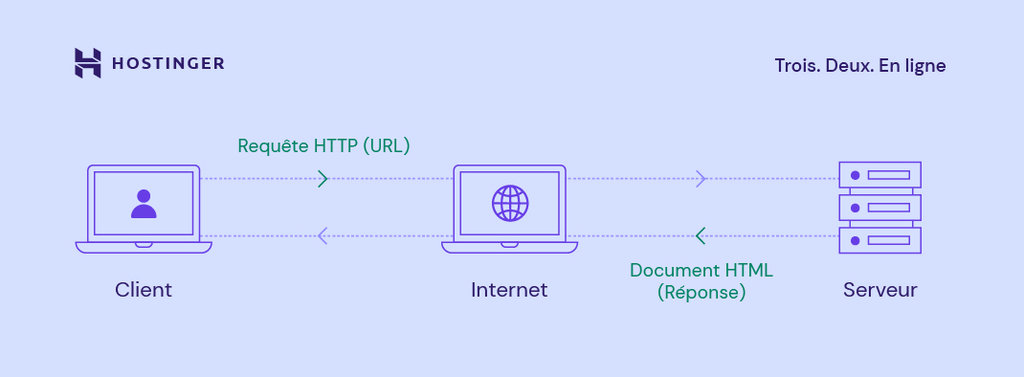
\includegraphics[width=0.6\textwidth]{PhotoMemoire/serveurweb_fonct.jpg}
\end{center}
	\caption{Fonctionnement d'un serveur Web\cite{3}}
\end{figure}

Les serveurs web suivent un modèle client-serveur. Dans cette structure, un programme, également appelé client, demande une ressource ou un service à un autre programme, le serveur.\\

Pour traiter les requêtes des clients web, les serveurs web suivent quelques étapes nécessaires :

\begin{enumerate}
\item Lorsqu’un internaute souhaite charger le contenu d’un site web, son navigateur web demande l’accès via Internet. C’est ce qu’on appelle une requête HTTP. Le navigateur web recherche l’adresse IP du site internet demandé en traduisant l’URL des pages web via le Système de Noms de Domaines (DNS) ou en cherchant dans son cache. Ce processus localise le serveur web sur lequel les fichiers du site internet sont hébergés.
\item  Le serveur web reçoit la requête HTTP et la traite via son serveur HTTP. Une fois que son serveur HTTP accepte la requête, il effectue une recherche dans les fichiers du serveur afin d’obtenir les données requises du site internet.

\item  Après cela, le serveur web renvoie les fichiers du site au navigateur web qui a envoyé la demande. Ensuite, l’internaute voit le contenu des pages web.\\


\end{enumerate}
Cependant, si le serveur HTTP ne parvient pas à trouver ou à traiter les fichiers demandés sur le serveur, il répond au navigateur web par un message d’erreur.\\
L’une des plus courantes est une erreur 404. Toutefois, une erreur 403 peut également apparaître en cas de problèmes d’autorisation sur le serveur.
\begin{figure}[h]
	\begin{center}
		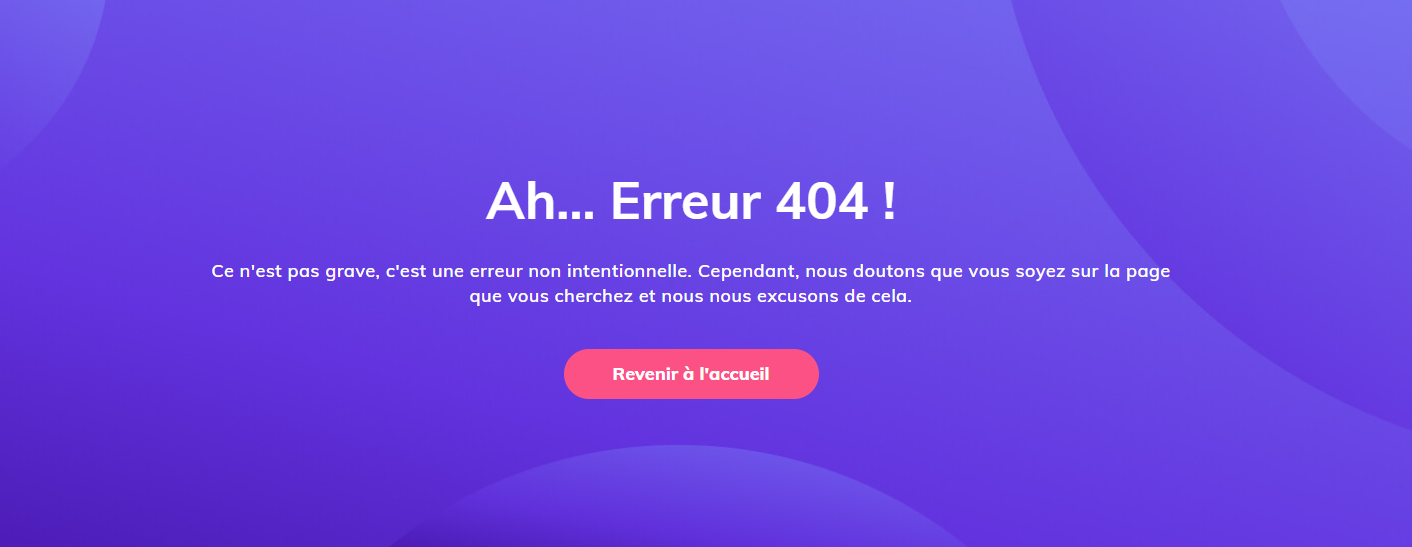
\includegraphics[width=0.6\textwidth]{PhotoMemoire/erruer404.png}
	\end{center}
	\caption{ Erreur 404\cite{3}}
\end{figure}

Si, par contre, un serveur web ne reçoit pas de réponse en temps opportun d’un autre serveur proxy agissant comme une passerelle, une erreur 504 se produit dans ce cas.
\subsection{Serveur web statique ou serveur web dynamique.}
Les serveurs web peuvent transmettre du contenu statique ou dynamique. Un serveur web statique se compose d’un ordinateur et d’un logiciel HTTP. Les serveurs web statiques renvoient les fichiers d’un site web à un navigateur web sans aucune modification.\\

Un serveur web dynamique comprend un serveur web statique et des logiciels supplémentaires. Ces logiciels se composent le plus souvent d’un serveur d’application et de bases de données.\\

Les serveurs web dynamiques mettent essentiellement à jour les fichiers hébergés avant de les diffuser via un serveur HTTP. Cela lui permet de générer et d’envoyer du contenu dynamique à un navigateur web.\\

\subsection{Fonctionnalités du serveur web}
Outre la prise en charge des protocoles HTTP pour traiter les demandes et les réponses entrantes, la plupart des serveurs web offrent les fonctionnalités standards suivantes :
\begin{enumerate}
	\item \textbf{ Journalisation des fichiers.\\} Les fichiers journaux documentent tous les événements ou activités que les serveurs web effectuent, tels que les requêtes, la sécurité et les erreurs. Chaque fois qu’un serveur web reçoit une nouvelle requête, une ligne de texte est ajoutée au journal.
	 
	 \item \textbf{ Authentification.\\} De nombreux serveurs offrent cette fonctionnalité avant d’autoriser un accès partiel ou complet aux ressources d’un site web. Les fonctions d’authentification impliquent souvent des demandes d’autorisation. Cela se produit lorsqu’un nom d’utilisateur et un mot de passe sont requis.
	 
	 \item \textbf{Limitation de la bande passante.\\} La bande passante d’un serveur web est la quantité de données qu’il peut transférer ou traiter à un moment donné. La limitation de la bande passante contrôle la vitesse des réponses pour s’assurer qu’un réseau n’est pas saturé et peut livrer les fichiers sans problèmes.
	 
	 \item \textbf{ Espace de stockage.\\} Il fait référence à la quantité d’espace disque disponible pour stocker des fichiers. Il détermine par conséquent si un serveur web peut héberger un site internet avec des caractéristiques spécifiques.
	 Un serveur web comprend d’autres éléments essentiels, tels que :
	 \begin{enumerate}
	 \item \textbf{Langage de programmation.\\} Le langage de programmation d’un serveur web est le type de code utilisé pour développer des programmes exécutés par un serveur. Il est également connu sous le nom de langages de script côté serveur. PHP et Python sont des exemples de langages de programmation très populaires.
	 \item \textbf{Disponibilité.\\} La disponibilité du serveur suit la durée pendant laquelle un serveur web est fonctionnel et peut traiter les demandes ou fournir des fichiers. \\
	 \subitem La disponibilité d’un serveur affecte aussi le moment où un site web hébergé est opérationnel. C’est ce que l’on appelle la disponibilité du site web. La norme de l’industrie est une garantie de 99,9 Pour-cent.
	\end{enumerate}
\end{enumerate}
\subsection{A quoi sert un serveur web ?}
Les serveurs web ont trois fonctions principales, lesquelles sont :
\begin{enumerate}
    	\item  Héberger plusieurs sites web ou applications web.,
	    \item  Traiter les demandes de Protocole de transfert de fichiers (FTP),
	    \item  Envoyer et recevoir des e-mails.
\end{enumerate}
Les serveurs web hébergent des sites internet afin qu’ils soient accessibles sur Internet. C’est pourquoi les caractéristiques et les fonctions d’un serveur web se concentrent sur la création et la maintenance d’un environnement d’hébergement.\\
Si vous souhaitez créer et publier un site web, vous devez avoir accès à un serveur web. Le moyen le plus pratique de le faire est de passer par les hébergeurs de sites.\\
L’hébergement web est un service qui fournit à votre site web un espace serveur pour stocker ses fichiers, scripts et bases de données. Consultez notre guide sur l’hébergement web pour en savoir plus.\\
En plus de tout cela, le rôle d’un fournisseur d’hébergement web est également de s’assurer que les serveurs fonctionnent de manière transparente. Cela implique d’effectuer des sauvegardes, la mise en cache, la surveillance de la sécurité et la maintenance générale. D’ailleurs, c’est pourquoi il est crucial de choisir un hébergeur fiable.\\
Certains des principaux avantages d’avoir un hébergeur web pour surveiller et maintenir le serveur web sur lequel votre site internet est hébergé sont les suivants :
\begin{enumerate}
	
	\item[$\bullet$]\textbf{Disponibilité et performances optimales.\\} Un hébergeur web s’occupe de la maintenance du matériel et des mises à jour logicielles, ce qui contribue à améliorer les performances et la disponibilité du site web.
 	\item [$\bullet$]\textbf{Serveurs sécurisés.\\} Les hébergeurs web mettent en œuvre des protocoles de sécurité efficaces pour réduire les vulnérabilités et protéger les sites hébergés contre les logiciels malveillants ou les cyberattaques.
	\item[$\bullet$]\textbf{Diverses options de plans d’hébergement.\\} Les propriétaires de sites peuvent choisir un plan d’hébergement web avec différentes caractéristiques et fonctions de leurs besoins.
	\item[$\bullet$] \textbf{Rentabilité.\\} Les propriétaires de sites n’ont pas à maintenir un serveur dédié et peuvent à la place opter pour un plan d’hébergement qui fournit la quantité nécessaire de ressources du serveur.
	\item [$\bullet$]\textbf{Flexibilité.} Les hébergeurs web proposent des plans évolutifs afin que les propriétaires de sites web puissent obtenir des ressources d’hébergement supplémentaires en fonction de leurs besoins. Il peut s’agir du stockage ou de la bande passante.
\end{enumerate}
\subsection{Serveurs web sur le marché}
Certains des exemples les plus populaires de serveurs web englobent :
\begin{enumerate}
	 \item [$\bullet$]\textbf{Serveur HTTP Apache.\\} Un serveur logiciel gratuit et open source maintenu par Apache Software Foundation et  utilisé pour de nombreux systèmes d’exploitation, y compris Windows, Linux et Mac OS X.\\
	 Apache est le plus ancien logiciel de serveur web et l’un des incontournables pour les propriétaires de sites web, les développeurs et les hébergeurs. Il dispose d’une part de marché de plus de 31 Pourcentage.
	 \item [$\bullet$]\textbf{NGINX.\\} Un célèbre logiciel de serveur web open source qui ne fonctionnait initialement que pour le service web HTTP. Il est désormais également utilisé comme proxy inverse, équilibreur de charge HTTP et proxy de messagerie. NGINX est apprécié pour sa rapidité et sa capacité à gérer plusieurs connexions. C’est pourquoi de nombreux sites à fort trafic font recours à ses services.
	 \item [$\bullet$]\textbf{Microsoft Internet Information Services (IIS).\\} IIS est un logiciel de serveur web à code source fermé et développé par Microsoft. Il est largement utilisé dans les systèmes d’exploitation Windows.
	 \item [$\bullet$]\textbf{Lighttpd.\\} Un logiciel de serveur web gratuit et open source connu pour sa vitesse tout en nécessitant moins de puissance CPU. Lighttpd est également populaire pour avoir une petite empreinte mémoire.
\end{enumerate}
\section*{Conclusion}
Un serveur web est un ordinateur qui stocke, traite et fournit des fichiers de sites. Il se compose d’un côté matériel et d’un côté logiciel (serveur http), chacun jouant un rôle distinct dans le traitement des fichiers.
\subsection{Quelques vulnérabilités Sur Les Serveurs Web }
 
Il y a plusieurs vulnérabilités qui peuvent affecter un serveur web, en voici quelques exemples :
\begin{itemize}
	 \item[$\bullet$] Injection SQL : Cette vulnérabilité permet à un attaquant d'injecter du code SQL malveillant dans une requête pour détourner le contrôle de la base de données.
	 \item[$\bullet$] Cross-site scripting (XSS) : Cette vulnérabilité permet à un attaquant d'injecter du code malveillant dans une page Web pour voler des informations d'authentification ou d'autres données sensibles.
	 \item[$\bullet$] Vulnérabilités du serveur HTTP : Les serveurs HTTP tels que Apache, Nginx et IIS peuvent être vulnérables à des attaques telles que les dénis de service (DoS) et les dénis de service distribués (DDoS).
	\item[$\bullet$] Mauvaise configuration : Une mauvaise configuration du serveur web peut permettre aux attaquants d'accéder aux fichiers sensibles ou d'exécuter du code malveillant.
	\item[$\bullet$] Vulnérabilités du CMS : Les systèmes de gestion de contenu tels que WordPress et Drupal peuvent être vulnérables à des attaques telles que les injections SQL et les attaques de force brute.
	 
\end{itemize}

Il est important de mettre en place des mesures de sécurité adéquates pour protéger les serveurs web contre ces vulnérabilités potentielles, telles que la mise à jour régulière de la sécurité du système et l'utilisation de logiciels de sécurité pour détecter et prévenir les attaques potentielles. 
\\Les développeurs de sites web doivent également être conscients des meilleures pratiques de sécurité, telles que la validation des entrées utilisateur et l'utilisation de l'encodage pour se protéger contre les attaques XSS.\\
\section{Serveurs de Messageries} 
	\begin{figure}[h]
		\begin{center}
			
		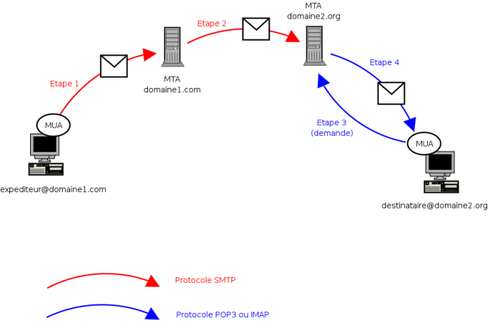
\includegraphics[width=0.8\textwidth]{PhotoMemoire/Serveur_Messagerie.png}
\caption{Schéma d'un Serveur de Messagerie \cite{7}}
	\end{center}
\end{figure}

Un serveur de messagerie est un type de serveur qui est utilisé pour envoyer et recevoir des courriers électroniques (e-mails). Les serveurs de messagerie sont essentiels pour le fonctionnement du courrier électronique car ils sont responsables de la distribution des messages entre les différents utilisateurs.\\

Il existe deux types principaux de serveurs de messagerie : le serveur SMTP (Simple Mail Transfer Protocol) et le serveur POP (Post Office Protocol).\\
\paragraph{ }
\textbf{Le serveur SMTP} est utilisé pour envoyer des courriers électroniques. Lorsqu'un utilisateur envoie un e-mail, le client de messagerie envoie le message au serveur SMTP, qui se charge de le transférer au serveur de messagerie du destinataire.\\

\textbf{Le serveur POP} est utilisé pour récupérer les courriers électroniques sur le serveur de messagerie. Les clients de messagerie utilisent le protocole POP pour se connecter au serveur de messagerie et récupérer les messages qui leur sont destinés.\\

Il existe également un autre protocole appelé IMAP (Internet Message Access Protocol) qui est utilisé pour accéder aux messages sur le serveur de messagerie sans les télécharger sur l'ordinateur local. IMAP permet aux utilisateurs de se connecter à leur boîte de réception depuis n'importe quel ordinateur ou appareil connecté à Internet.

Les serveurs de messagerie peuvent être configurés pour fournir des fonctionnalités supplémentaires telles que la sécurité des messages, la gestion des spams et des virus, la gestion des listes de diffusion, etc. Les serveurs de messagerie sont également souvent intégrés à des suites de collaboration pour permettre le partage de calendriers, de contacts, de tâches, etc.
\subsection{Quelques vulnérabilités Sur Les Serveurs de Messageries }
Il existe plusieurs vulnérabilités potentielles qui peuvent affecter les serveurs de messagerie. Voici quelques exemples :
\begin{itemize}
	\item[$\bullet$]Injection de code : Les attaquants peuvent exploiter des vulnérabilités dans le serveur de messagerie pour injecter du code malveillant dans les e-mails, qui peuvent ensuite être utilisés pour exécuter des attaques de phishing, des attaques de logiciels malveillants ou d'autres types d'attaques.
	
	
	\item[$\bullet$] Attaques de force brute : Les attaquants peuvent tenter de deviner les identifiants de connexion des utilisateurs en utilisant des attaques de force brute, qui impliquent l'utilisation de programmes pour tester toutes les combinaisons de noms d'utilisateur et de mots de passe possibles.
	
	
	\item[$\bullet$] Attaques par déni de service (DoS) : Les attaquants peuvent lancer des attaques par déni de service (DoS) contre le serveur de messagerie pour le rendre indisponible, ce qui peut empêcher les utilisateurs d'accéder à leurs e-mails ou de les envoyer.
	
	
	\item[$\bullet$]Vulnérabilités de sécurité : Les serveurs de messagerie peuvent avoir des vulnérabilités de sécurité connues qui peuvent être exploitées par les attaquants pour accéder à des données sensibles, tels que des courriels confidentiels ou des informations d'identification.
	
	
	\item[$\bullet$] Vulnérabilités de configuration : Les serveurs de messagerie peuvent avoir des vulnérabilités de configuration qui peuvent être exploitées par les attaquants pour accéder à des données sensibles, tels que des listes de contacts, des calendriers et des tâches.
	 
\end{itemize}

Il est important de mettre en place des mesures de sécurité adéquates pour protéger les serveurs de messagerie contre ces vulnérabilités potentielles, telles que la mise à jour régulière de la sécurité du système et l'utilisation de logiciels de sécurité pour détecter et prévenir les attaques potentielles.\\
 Les utilisateurs doivent également être éduqués sur les meilleures pratiques de sécurité, telles que la création de mots de passe forts et l'utilisation de l'authentification à deux facteurs pour protéger leurs comptes de messagerie.\\
\section{Serveur de fichiers} 
	\begin{figure}[h]
		\begin{center}
		
	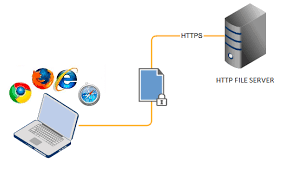
\includegraphics[width=0.8\textwidth]{PhotoMemoire/serveur_fichier.png}
\caption{Schéma De Serveur De Fichier\cite{7}}
\end{center}
\end{figure}
\paragraph{ }
Un serveur de fichiers est un type de serveur qui stocke des fichiers et des dossiers, et permet à des utilisateurs de les accéder et de les partager via un réseau. Les serveurs de fichiers peuvent être configurés pour fournir différentes fonctionnalités, telles que :
\begin{enumerate}
 \item[$\bullet$]  Partage de fichiers : Les utilisateurs peuvent accéder aux fichiers stockés sur le serveur et les partager avec d'autres utilisateurs du réseau.
 
 \item[$\bullet$]Gestion des droits d'accès : Les administrateurs peuvent définir des autorisations d'accès pour chaque utilisateur ou groupe d'utilisateurs, afin de contrôler qui peut accéder à quels fichiers.
 
\item[$\bullet$] Sauvegarde de données : Les serveurs de fichiers peuvent être configurés pour effectuer des sauvegardes régulières des fichiers stockés, afin de protéger les données contre la perte ou la corruption.
 
\item[$\bullet$]Synchronisation de fichiers : Les utilisateurs peuvent synchroniser des fichiers entre le serveur de fichiers et leur ordinateur local, pour assurer une cohérence des données.
 
\item[$\bullet$]Accès à distance : Les utilisateurs peuvent accéder aux fichiers stockés sur le serveur de fichiers à partir d'un emplacement distant en utilisant un client de connexion sécurisé.
 
  \item[$\bullet$] Stockage en nuage : Les serveurs de fichiers peuvent être configurés pour stocker des fichiers dans le cloud, ce qui permet aux utilisateurs d'y accéder à partir de n'importe où avec une connexion Internet.
 
\item[$\bullet$] Accès multiplateforme : Les serveurs de fichiers peuvent être configurés pour fournir un accès multiplateforme aux utilisateurs, ce qui permet aux utilisateurs d'accéder aux fichiers à partir de différents systèmes d'exploitation tels que Windows, Mac OS ou Linux.
 
\end{enumerate}
Les serveurs de fichiers sont couramment utilisés dans les entreprises pour stocker et partager des fichiers entre les employés, mais ils peuvent également être utilisés dans des environnements domestiques pour stocker et partager des fichiers entre les membres de la famille.
\subsection{Quelques vulnérabilités Sur Les Serveurs de Fichier}
Il existe plusieurs vulnérabilités potentielles qui peuvent affecter les serveurs de fichiers. Voici quelques exemples :

\begin{enumerate}
\item[$\bullet$]  Vulnérabilités de sécurité : Les serveurs de fichiers peuvent avoir des vulnérabilités de sécurité connues qui peuvent être exploitées par les attaquants pour accéder à des données sensibles, telles que des fichiers confidentiels ou des informations d'identification.
 
 \item[$\bullet$]  Vulnérabilités de configuration : Les serveurs de fichiers peuvent avoir des vulnérabilités de configuration qui peuvent être exploitées par les attaquants pour accéder à des données sensibles, telles que des fichiers de configuration ou des répertoires de fichiers.
 
\item[$\bullet$] Attaques par déni de service (DoS) : Les attaquants peuvent lancer des attaques par déni de service (DoS) contre le serveur de fichiers pour le rendre indisponible, ce qui peut empêcher les utilisateurs d'accéder aux fichiers hébergés sur ce serveur.
 
 \item[$\bullet$]  Attaques de force brute : Les attaquants peuvent tenter de deviner les identifiants de connexion des utilisateurs en utilisant des attaques de force brute, qui impliquent l'utilisation de programmes pour tester toutes les combinaisons de noms d'utilisateur et de mots de passe possibles.
 
\item[$\bullet$]  Fuites de données : Les serveurs de fichiers peuvent être vulnérables aux fuites de données, qui peuvent se produire lorsque des données sensibles sont stockées de manière inappropriée ou lorsque des utilisateurs non autorisés y ont accès.
\end{enumerate}

Il est important de mettre en place des mesures de sécurité adéquates pour protéger les serveurs de fichiers contre ces vulnérabilités potentielles, telles que la mise à jour régulière de la sécurité du système et l'utilisation de logiciels de sécurité pour détecter et prévenir les attaques potentielles.\\
 Les utilisateurs doivent également être éduqués sur les meilleures pratiques de sécurité, telles que la création de mots de passe forts et l'utilisation de l'authentification à deux facteurs pour protéger leur accès aux fichiers stockés sur le serveur de fichiers.
\section{Serveur de Base de Données } 
	\begin{figure}[h]
		\begin{center}
	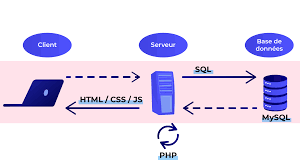
\includegraphics[width=0.8\textwidth]{PhotoMemoire/serveur_bdd.png}
\caption{Schema De Serveur De Base De Données \cite{6}}
\end{center}
\end{figure}
Un serveur de base de données est un type de serveur qui stocke des données et fournit des services pour gérer ces données. Il permet aux utilisateurs de stocker, d'organiser, d'accéder et de gérer des données de manière efficace et sécurisée.
\paragraph{ }
Les serveurs de base de données sont utilisés pour stocker des informations sur des produits, des clients, des transactions financières, des employés, des stocks, etc. Ils sont également utilisés pour alimenter des applications qui nécessitent un accès rapide et efficace aux données, telles que les sites web, les applications mobiles, les systèmes de gestion de la relation client (CRM), les systèmes de gestion de la chaîne d'approvisionnement (SCM), etc.

Les serveurs de bases de données peuvent être configurés pour fournir différentes fonctionnalités, telles que :

\begin{enumerate}
	
 \item[$\bullet$] Langage de requête : Les serveurs de bases de données prennent en charge des langages de requête tels que SQL (Structured Query Language) pour interroger et récupérer les données stockées.
 
 \item[$\bullet$] Gestion des transactions : Les serveurs de bases de données prennent en charge la gestion des transactions pour garantir l'intégrité des données et éviter les conflits.
 
 \item[$\bullet$] Gestion des utilisateurs et des droits d'accès : Les administrateurs peuvent définir des autorisations d'accès pour chaque utilisateur ou groupe d'utilisateurs, afin de contrôler qui peut accéder à quelles données.
 
  \item[$\bullet$] Sauvegarde et restauration : Les serveurs de bases de données peuvent être configurés pour effectuer des sauvegardes régulières des données stockées, afin de protéger les données contre la perte ou la corruption.
 
\item[$\bullet$] Réplication des données : Les serveurs de bases de données peuvent être configurés pour répliquer les données sur plusieurs serveurs, pour améliorer la disponibilité et la redondance des données.
 
 \item[$\bullet$] Sécurité des données : Les serveurs de bases de données peuvent être configurés pour fournir des fonctionnalités de sécurité avancées, telles que le chiffrement des données, l'authentification à deux facteurs, etc.
 
\end{enumerate}

Les serveurs de bases de données sont couramment utilisés dans les entreprises pour stocker et gérer des données importantes, mais ils peuvent également être utilisés dans des environnements domestiques pour stocker et gérer des données personnelles telles que les finances, les contacts, les photos, etc.

\subsection{Quelques vulnérabilités Sur Les Serveurs de Base De Donnes }

Il existe plusieurs vulnérabilités potentielles qui peuvent affecter les serveurs de bases de données. Voici quelques exemples :
\begin{enumerate}



\item[$\bullet$] Injection SQL : Les attaquants peuvent exploiter des vulnérabilités dans le serveur de base de données pour injecter du code SQL malveillant, qui peut permettre aux attaquants de prendre le contrôle du serveur de base de données, de modifier ou de supprimer des données, ou encore d'accéder à des informations confidentielles.
	
\item[$\bullet$]  Vulnérabilités de sécurité : Les serveurs de bases de données peuvent avoir des vulnérabilités de sécurité connues, telles que la configuration par défaut de mots de passe faibles, qui peuvent être exploitées par les attaquants pour accéder à des données sensibles.
	
\item[$\bullet$]  Attaques par déni de service (DoS) : Les attaquants peuvent lancer des attaques par déni de service (DoS) contre le serveur de base de données pour le rendre indisponible, ce qui peut empêcher les utilisateurs d'accéder aux données stockées sur ce serveur.
	
\item[$\bullet$] Vulnérabilités de configuration : Les serveurs de bases de données peuvent avoir des vulnérabilités de configuration qui peuvent être exploitées par les attaquants pour accéder à des données sensibles, telles que des informations de connexion ou des fichiers de configuration.
	
\item[$\bullet$]  Fuites de données : Les serveurs de bases de données peuvent être vulnérables aux fuites de données, qui peuvent se produire lorsque des données sensibles sont stockées de manière inappropriée ou lorsque des utilisateurs non autorisés y ont accès.
\end{enumerate}
Il est important de mettre en place des mesures de sécurité adéquates pour protéger les serveurs de bases de données contre ces vulnérabilités potentielles, telles que la mise à jour régulière de la sécurité du système et l'utilisation de logiciels de sécurité pour détecter et prévenir les attaques potentielles. Les développeurs de bases de données doivent également être conscients des meilleures pratiques de sécurité, telles que la validation des entrées utilisateur et l'utilisation de l'authentification à deux facteurs pour protéger l'accès aux données stockées sur le serveur de bases de données.
\section{Serveur d'Application} 
	\begin{figure}[h]
	\begin{center}	
	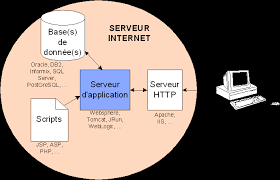
\includegraphics[width=0.8\textwidth]{PhotoMemoire/serveur_application.png}
\caption{Schéma D'un serveur D'application\cite{7}}
\end{center}
\end{figure}
Un serveur d'application est un type de serveur qui héberge des applications et fournit des services d'application aux clients. Les serveurs d'application sont essentiels pour les entreprises qui développent et déploient des applications commerciales, car ils fournissent une plateforme pour exécuter et gérer ces applications de manière efficace et sécurisée.\\

Les serveurs d'application peuvent être utilisés pour héberger une grande variété d'applications, telles que les applications de commerce électronique, les applications de gestion de contenu, les applications de gestion de la relation client (CRM), les applications de gestion de la chaîne d'approvisionnement (SCM), les applications de collaboration, etc.\\

Les serveurs d'application peuvent fournir différentes fonctionnalités, telles que :
\begin{enumerate}
	\item[$\bullet$]Gestion de la connectivité : Les serveurs d'application peuvent gérer la connectivité entre les applications et les différents systèmes d'information, tels que les bases de données, les systèmes de fichiers, les services web, etc.
	 
	\item[$\bullet$] Gestion des transactions : Les serveurs d'application peuvent gérer les transactions pour garantir l'intégrité des données et éviter les conflits.
	 
	\item[$\bullet$] Gestion de la sécurité : Les serveurs d'application peuvent fournir des fonctionnalités de sécurité avancées pour protéger les applications et les données contre les menaces potentielles.
	 
	 \item[$\bullet$] Gestion des sessions : Les serveurs d'application peuvent gérer les sessions pour assurer la continuité des services aux utilisateurs lorsqu'ils passent d'une page à l'autre ou lorsqu'ils se connectent à l'application à partir de différents appareils.
	 
	\item[$\bullet$] Gestion des performances : Les serveurs d'application peuvent surveiller et optimiser les performances de l'application pour assurer une expérience utilisateur rapide et fluide.
	 
\end{enumerate}
Les serveurs d'application sont souvent utilisés en conjonction avec d'autres outils de développement et de déploiement, tels que les serveurs web, les bases de données, les outils de développement intégrés (IDE), les systèmes de contrôle de version, etc.\\
\subsection{Quelques vulnérabilités Sur Les Serveurs d'Application }
Il existe plusieurs vulnérabilités potentielles qui peuvent affecter les serveurs d'application. Voici quelques exemples :
\begin{enumerate}
\item[$\bullet$]  Vulnérabilités de sécurité : Les serveurs d'application peuvent avoir des vulnérabilités de sécurité connues, telles que des failles dans les algorithmes de chiffrement ou des vulnérabilités dans les bibliothèques tierces, qui peuvent être exploitées par les attaquants pour accéder à des données sensibles ou prendre le contrôle du serveur.

\item[$\bullet$]  Attaques par déni de service (DoS) : Les attaquants peuvent lancer des attaques par déni de service (DoS) contre le serveur d'application pour le rendre indisponible, ce qui peut empêcher les utilisateurs d'accéder aux applications hébergées sur ce serveur.

\item[$\bullet$]  Injection de code : Les attaquants peuvent exploiter des vulnérabilités dans le serveur d'application pour injecter du code malveillant dans les applications, qui peuvent ensuite être utilisées pour exécuter des attaques de phishing, des attaques de logiciels malveillants ou d'autres types d'attaques.

\item[$\bullet$] Vulnérabilités de configuration : Les serveurs d'application peuvent avoir des vulnérabilités de configuration qui peuvent être exploitées par les attaquants pour accéder à des données sensibles, telles que des informations de connexion ou des fichiers de configuration.

\item[$\bullet$]  Fuites de données : Les serveurs d'application peuvent être vulnérables aux fuites de données, qui peuvent se produire lorsque des données sensibles sont stockées de manière inappropriée ou lorsque des utilisateurs non autorisés y ont accès.
\end{enumerate}
Il est important de mettre en place des mesures de sécurité adéquates pour protéger les serveurs d'application contre ces vulnérabilités potentielles, telles que la mise à jour régulière de la sécurité du système et l'utilisation de logiciels de sécurité pour détecter et prévenir les attaques potentielles.\\
 Les développeurs d'applications doivent également être conscients des meilleures pratiques de sécurité, telles que la validation des entrées utilisateur et l'utilisation de l'authentification à deux facteurs pour protéger les applications hébergées sur le serveur d'application.\\
 
 \section{Serveur DNS} 
	\begin{figure}[h]
		\begin{center}
	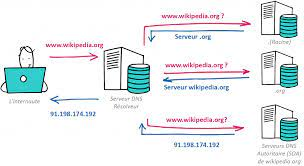
\includegraphics[width=0.8\textwidth]{PhotoMemoire/serveur_dns.jpeg}
	\caption{Schéma d'un Serveur DNS\cite{7}}
\end{center}
\end{figure}

Un serveur DNS (Domain Name System) est un type de serveur qui permet de traduire les noms de domaine en adresses IP. Les noms de domaine sont des identificateurs textuels, tels que "google.com" ou "facebook.com", qui sont plus faciles à mémoriser que les adresses IP numériques qui identifient les ordinateurs et les serveurs sur Internet.\\

Lorsqu'un utilisateur entre un nom de domaine dans son navigateur web, le navigateur envoie une requête DNS au serveur DNS pour obtenir l'adresse IP correspondante. Le serveur DNS répond alors avec l'adresse IP, qui est utilisée pour établir la connexion avec le serveur web correspondant.\\

Les serveurs DNS sont essentiels pour le fonctionnement d'Internet, car ils permettent aux utilisateurs d'accéder aux sites web et aux services en ligne en utilisant des noms de domaine plutôt que des adresses IP numériques. Les serveurs DNS sont également utilisés pour acheminer le courrier électronique et pour fournir d'autres services de réseau.\\

Les serveurs DNS peuvent être configurés pour fournir différentes fonctionnalités, telles que :

 \begin{enumerate}
	
	\item[$\bullet$]     Caching de requêtes : Les serveurs DNS peuvent mettre en cache les réponses aux requêtes DNS précédentes pour accélérer les temps de réponse et réduire la charge sur le réseau.
	 
\item[$\bullet$] Résolution de noms de domaine : Les serveurs DNS peuvent résoudre les noms de domaine en adresses IP en utilisant des bases de données de noms de domaine et des serveurs racines.
	 
	 \item[$\bullet$] Redirection de domaine : Les serveurs DNS peuvent être configurés pour rediriger les requêtes vers d'autres serveurs DNS, en fonction des besoins.
	 
	 \item[$\bullet$] Sécurité DNS : Les serveurs DNS peuvent implémenter des fonctionnalités de sécurité avancées, telles que DNSSEC (DNS Security Extensions), pour protéger contre les attaques de DNS spoofing et de DNS cache poisoning.
	 
	 \item[$\bullet$] Load balancing : Les serveurs DNS peuvent être utilisés pour répartir la charge entre plusieurs serveurs web en redirigeant les requêtes vers différents serveurs en fonction des besoins.
	 
\end{enumerate}

Les serveurs DNS sont souvent gérés par les fournisseurs de services Internet (ISP), les entreprises et les organisations gouvernementales. Les utilisateurs peuvent également configurer leur propre serveur DNS pour fournir une résolution de noms de domaine personnalisée ou pour améliorer la sécurité et la performance de leur réseau local.
\subsection{Quelques vulnérabilités Sur Les Serveurs DNS }

Il existe plusieurs vulnérabilités potentielles qui peuvent affecter les serveurs de DNS (Domain Name System). Voici quelques exemples :\\

\begin{enumerate}
	\item[$\bullet$] Attaques par déni de service (DoS) : Les attaquants peuvent lancer des attaques par déni de service (DoS) contre le serveur de DNS pour le rendre indisponible, ce qui peut empêcher les utilisateurs d'accéder aux noms de domaine associés à ce serveur.
	
	 \item[$\bullet$] Vulnérabilités de sécurité : Les serveurs de DNS peuvent avoir des vulnérabilités de sécurité connues qui peuvent être exploitées par les attaquants pour accéder à des données sensibles, telles que des informations de connexion ou des fichiers de configuration.
	
\item[$\bullet$]  Attaques de cache poisoning : Les attaquants peuvent exploiter des vulnérabilités dans le serveur de DNS pour modifier le contenu du cache DNS, ce qui peut rediriger les utilisateurs vers des sites web malveillants.
	
	\item[$\bullet$]  Vulnérabilités de configuration : Les serveurs de DNS peuvent avoir des vulnérabilités de configuration qui peuvent être exploitées par les attaquants pour accéder à des données sensibles, telles que des informations de connexion ou des fichiers de configuration.
	
\item[$\bullet$] Fuites de données : Les serveurs de DNS peuvent être vulnérables aux fuites de données, qui peuvent se produire lorsque des données sensibles sont stockées de manière inappropriée ou lorsque des utilisateurs non autorisés y ont accès.
	
\end{enumerate}

Il est important de mettre en place des mesures de sécurité adéquates pour protéger les serveurs de DNS contre ces vulnérabilités potentielles, telles que la mise à jour régulière de la sécurité du système et l'utilisation de logiciels de sécurité pour détecter et prévenir les attaques potentielles. Les administrateurs de DNS doivent également être conscients des meilleures pratiques de sécurité, telles que la mise en place de politiques de sécurité strictes pour l'accès au serveur de DNS et la configuration correcte du serveur de DNS pour minimiser les risques d'attaques de cache poisoning.
 
\section{Serveur de Jeu} 
	\begin{figure}[h]
		\begin{center}
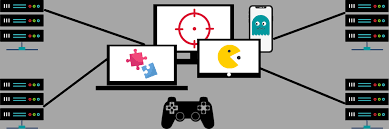
\includegraphics[width=0.8\textwidth]{PhotoMemoire/serveur_jeux.png}
\caption{Un Schema de Serveur de Jeu \cite{7}}
	\end{center}
	\end{figure}
		
Un serveur de jeu est un type de serveur qui permet de fournir des services de jeu en ligne à des joueurs du monde entier. Les serveurs de jeu sont utilisés pour héberger des jeux multijoueurs en ligne, tels que les jeux de tir à la première personne, les jeux de stratégie en temps réel, les jeux de rôle en ligne massivement multijoueurs (MMORPG), les jeux de sport en ligne, etc.

Les serveurs de jeu offrent des fonctionnalités telles que :
\begin{enumerate}
	
  \item[$\bullet$] Hébergement de jeux multijoueurs : Les serveurs de jeu sont utilisés pour héberger des jeux multijoueurs en ligne pour permettre aux joueurs de jouer ensemble sur Internet.
 
\item[$\bullet$]  Gestion des joueurs : Les serveurs de jeu peuvent gérer les joueurs, les scores, les classements et les statistiques de jeu, ainsi que les opérations de modération pour assurer un environnement de jeu sécurisé et équitable.
 
\item[$\bullet$] Optimisation des performances : Les serveurs de jeu peuvent être optimisés pour offrir des performances de jeu optimales, telles que des temps de latence réduits et une faible latence pour une expérience de jeu fluide.
 
\item[$\bullet$]  Gestion de la bande passante : Les serveurs de jeu peuvent gérer la bande passante pour optimiser les performances de jeu et éviter les problèmes de lag ou de décalage.
 
\item[$\bullet$]  Gestion des mises à jour : Les serveurs de jeu peuvent gérer les mises à jour de jeu pour maintenir les joueurs à jour avec les dernières fonctionnalités et correctifs de bugs.
 
\end{enumerate}

Les serveurs de jeu sont utilisés par les développeurs de jeux pour héberger leurs jeux en ligne et fournir des services de jeu en ligne à des millions de joueurs dans le monde entier. Les serveurs de jeu peuvent être exploités directement par les développeurs de jeux ou par des fournisseurs de services tiers spécialisés dans l'hébergement de serveurs de jeu. Les serveurs de jeu sont essentiels pour les jeux multijoueurs en ligne, car ils permettent aux joueurs de jouer ensemble sur Internet, offrant ainsi une expérience de jeu immersive et sociale.
 

Il existe plusieurs vulnérabilités potentielles qui peuvent affecter les serveurs de jeu. Voici quelques exemples :
\begin{enumerate}
\item[$\bullet$]  Vulnérabilités de sécurité : Les serveurs de jeu peuvent avoir des vulnérabilités de sécurité connues qui peuvent être exploitées par les attaquants pour accéder à des données sensibles, telles que des informations de compte de joueur ou des données de paiement.
	
	\item[$\bullet$] Attaques par déni de service (DoS) : Les attaquants peuvent lancer des attaques par déni de service (DoS) contre le serveur de jeu pour le rendre indisponible, ce qui peut empêcher les joueurs d'accéder au jeu ou de jouer en ligne.
	
\item[$\bullet$]  Exploits de jeu : Les attaquants peuvent exploiter des vulnérabilités dans le code du jeu pour gagner un avantage injuste sur les autres joueurs, ou pour perturber le jeu pour tous les autres joueurs.
	
\item[$\bullet$]  Vulnérabilités de configuration : Les serveurs de jeu peuvent avoir des vulnérabilités de configuration qui peuvent être exploitées par les attaquants pour accéder à des données sensibles, telles que des informations de connexion ou des fichiers de configuration.
	
\item[$\bullet$] Fuites de données : Les serveurs de jeu peuvent être vulnérables aux fuites de données, qui peuvent se produire lorsque des données sensibles sont stockées de manière inappropriée ou lorsque des utilisateurs non autorisés y ont accès.
\end{enumerate}
Il est important de mettre en place des mesures de sécurité adéquates pour protéger les serveurs de jeu contre ces vulnérabilités potentielles, telles que la mise à jour régulière de la sécurité du système et l'utilisation de logiciels de sécurité pour détecter et prévenir les attaques potentielles. Les développeurs de jeux doivent également être conscients des meilleures pratiques de sécurité, telles que la validation des entrées utilisateur et l'utilisation de l'authentification à deux facteurs pour protéger les comptes de joueur. Les administrateurs de serveurs de jeu doivent également surveiller les activités suspectes et mettre en place des politiques de sécurité strictes pour minimiser les risques d'attaques.

 \section*{\underline{Constat}}
 Si vous remarquez  bien que sur tout les serveurs que je viens de citer nous voyons que les attaques comme :
 \begin{enumerate}
 	\item[$\bullet$] L'attaque Par Déni de Service (DoS).
 	\item[$\bullet$] Vulnérabilité de Configuration.
 	\item[$\bullet$] Fuites de données.
 	\item[$\bullet$] Vulnérabilité de Sécurité  .
 \end{enumerate}
 
Dans ce le chapitre qui suit nous allons essayer de parler des méthodes,  manières par lesquelles nous pouvons éviter de tomber  dans les pièges d'attaques citées ci-hauts .

\chapter{La Cybersécurité et La Sécurité Informatique}
\section{La Cybersécurité}
\subsection{Définition}

La racine « \textbf{cyber} » provient du mot cybernétique, qui avait été formé en français
en 1834 pour désigner la «\textbf{ science du gouvernement} », à partir du grec Kubernêtiké, signifiant « \textbf{diriger, gouverner} ».\\
Terme repris en 1948, par le mathématicien Norman Wiener aux États-Unis à l’origine de la cybernétique (cybernetics), science constituée par l’ensemble des théories relatives au contrôle, à la régulation et à la communication entre l’être vivant et la machine.\\
La cybersécurité, également appelée sécurité informatique ou sécurité des technologies de l'information, est l'ensemble des mesures techniques, organisationnelles et juridiques mises en place pour protéger les systèmes informatiques, les réseaux et les données contre les attaques, les pertes ou les altérations.\\
 Elle vise à garantir la confidentialité, l'intégrité et la disponibilité des informations stockées sur les systèmes informatiques, ainsi que la protection de la vie privée et des droits de propriété intellectuelle.\\

La cybersécurité concerne la sécurité informatique et des réseaux des environnements connectés à Internet et accessibles via le cyberespace.\\
 Elle peut être mise en défaut, entre autres, par des cyberattaques informatiques.\\
 Du fait de l’usage extensif d’Internet, de nouvelles menaces sont apparues générant des risques additionnels dont les impacts, de niveaux d’importance variables, peuvent affecter les individus, les organisations ou les États.\\ 

La cybersécurité est devenue un enjeu majeur dans le monde numérique d'aujourd'hui, où les attaques informatiques sont de plus en plus sophistiquées et fréquentes.\\
 Elle est essentielle pour protéger les systèmes informatiques et les données sensibles contre les menaces potentielles et assurer la continuité des activités des organisations qui les utilisent.\\
  La cybersécurité est également importante pour protéger les utilisateurs finaux, tels que les consommateurs et les employés, contre les risques de vol d'identité, de fraude en ligne et d'autres formes de cybercriminalité.\\
Le préfixe « Cyber » est relatif à l’environnement informatique et aux activités
rendues possibles par les technologies du numérique et de l’Internet.\\
 Le cyberespace (l’ensemble des infrastructures numériques, des données et des services mis en réseaux) est une extension de notre espace naturel qui reflète notre société avec ses réalités politique, économique, sociale et culturelle.\\
  Mais contrairement à la terre, à la mer, à l’air et à l’espace-extra atmosphérique, le cyberespace est une pure création de l’être humain qui ne relève pas de la nature.\\

Les points essentiels englobés par la cybersécurité comprennent :
\space 
 
 \paragraph{1. La confidentialité :\\}la protection des données contre les accès non autorisés. Cela inclut la protection des données personnelles, des secrets commerciaux, des informations financières et autres informations sensibles.

 \paragraph{2. L'intégrité :\\}  la protection des données contre les altérations non autorisées. Cela inclut la garantie que les données sont exactes et fiables.

 \paragraph{3. La disponibilité :\\}  la garantie que les systèmes, les réseaux et les données sont accessibles et fonctionnent correctement, et que les interruptions de service sont minimisées.

 \paragraph{4. L'authenticité:\\} la garantie que les utilisateurs sont bien ceux qu'ils prétendent être, et que les données sont bien celles qu'elles prétendent être.

 \paragraph{5. La non-répudiation:\\} la garantie qu'une personne ne peut pas nier avoir effectué une action ou avoir envoyé des données.

 \paragraph{6. La résilience :\\} la capacité des systèmes et des réseaux à résister aux attaques et à récupérer rapidement en cas d'incident.


 \paragraph{7. La conformité :\\} le respect des lois, des réglementations et des normes en matière de sécurité informatique.

 \paragraph{8. La sensibilisation :\\} l'éducation et la formation des utilisateurs pour qu'ils comprennent les risques liés à la sécurité informatique et les meilleures pratiques à suivre pour les éviter.
 
Ces points essentiels sont inter-connectés et doivent être pris en compte dans toute stratégie de cybersécurité efficace.\\
\subsection{Pourquoi la cybersécurité est-elle nécessaire ?}
En 2021, le cybercrime a coûté au monde 6 000 milliards de dollars américains. D’ici 2025, ce coût passera à 10500 milliards de dollars.\\
 Le cybercrime est un problème de plus en plus sérieux, et pour s’y attaquer, il est essentiel de disposer d’un excellent dispositif de cybersécurité.\\

Les individus, les gouvernements, les entreprises, les organismes à but non lucratif et les établissements d’enseignement risquent tous de subir des cyberattaques et des violations de données.\\
 À l’avenir, le nombre d’attaques se multipliera, avec l’évolution des technologies numériques, l’augmentation du nombre d’appareils et d’utilisateurs, les chaînes logistiques mondiales de plus en plus complexes, et le rôle de plus en plus stratégique des données dans l’économie numérique.\\
  Pour minimiser le risque d’une attaque et pour sécuriser les systèmes et les données, un solide dispositif de cybersécurité devient vital.\\
\subsection{Comment les risques de cybersécurité sont-ils mesurés ?}
Le risque de cybersécurité correspond au potentiel de perte ou de préjudice résultant de l’endommagement d’une ressource informatique, susceptible d’entraîner un vol de propriété intellectuelle, une perte financière, une atteinte à la réputation, et des amendes légales ou réglementaires. En mesurant les risques, les entreprises peuvent optimiser les actions permettant de mieux les gérer, et s’assurer ainsi qu’il n’y a pas d’obstacles aux objectifs commerciaux.\\

\textbf{Identifier les ressources et définir leur priorité.} L’évaluation des risques de cybersécurité commence par la compréhension des ressources de l’entreprise et la définition de leur priorité, en établissant celles dont la perte, l’exposition ou l’endommagement pourrait avoir un impact sur les opérations.\\

\textbf{Identifier les vulnérabilités.}
 Toutes les vulnérabilités susceptibles de laisser une menace causer des dommages sont identifiées à l’aide de l’analyse automatique des vulnérabilités, des tests d’intrusion, ou de l’utilisation d’une base de données de vulnérabilités telle que la  \href{https://nvd.nist.gov/}{base de données nationale des vulnérabilités du NIST.}\\
 
 \textbf{Calculer l’impact de la menace.} L’impact probable ou le dommage que pourrait causer une menace à une ressource est calculé et classé comme élevé, moyen ou faible.\\
 \textbf{Calculer le risque.}Risque = Menace x Vulnérabilité x Ressource. À partir de cette équation, l’entreprise peut mesurer chaque risque.\\
\textbf{ Créer une matrice de risques pour la planification des corrections.} Enfin, la matrice de risques est établie, les deux axes représentant la probabilité et l’impact.\\

\textbf{Risque = Probabilité x Impact.} À partir de cette valeur, chaque risque est classé comme élevé, moyen ou faible, à la suite de quoi les stratégies de réduction appropriées sont mises en œuvre.\\
	
	 
	 
\begin{figure}[h]
	\begin{center}
	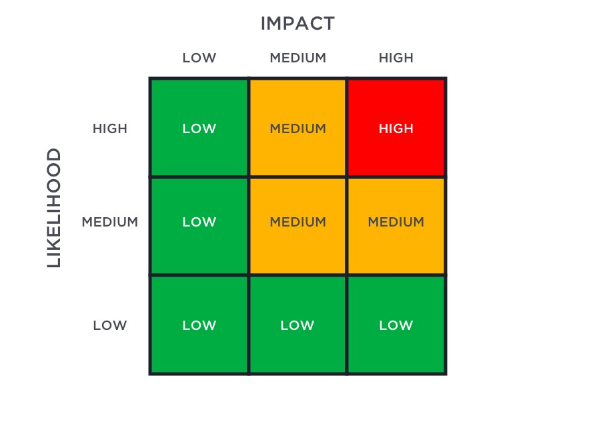
\includegraphics[width=0.7\textwidth]{PhotoMemoire/tableauImpact.png}
\caption{Un Tableau Illustrant Les Impact \cite{15}}
\end{center}
\end{figure}

\subsection{Cybersécurité avfondeur (DEP)}
Il n’existe pas de méthode ou d’outil de cybersécurité capable de défendre de tous les types d’attaque. Voilà pourquoi la cybersécurité avec défense en profondeur (DEP) est essentielle.\\
Avec la DEP, également connue sous le nom d’ « approche forteresse » en matière de cybersécurité, des mécanismes défensifs multiples sont mis en œuvre pour protéger les ressources d’entreprise.\\
Cette approche multicouche renforce la sécurité globale. De plus, si un mécanisme échoue, les autres fonctionneront pour prévenir ou stopper les cyberattaques.\\

Une stratégie de cybersécurité avec DEP inclut différents éléments :\\

\textbf{Logiciel antivirus.} 
Les solutions antivirus comportant des fonctionnalités heuristiques qui recherchent et signalent les activités suspectes offrent une plus forte protection que les solutions classiques basées sur des signatures.\\

\textbf{Contrôles de sécurité du réseau.} 
Les pare-feu et les systèmes de protection contre les intrusions peuvent identifier des menaces de sécurité potentielles, et les bloquer à partir de règles de sécurité.\\

\textbf{Solutions d’intégrité des données.}
Ces produits vérifient les adresses IP sources pour confirmer que les fichiers entrants proviennent de sources connues et de confiance uniquement.\\

	\textbf{Analyse comportementale.} Ces systèmes analysent les comportements des fichiers et des réseaux en fonction de comportements « normaux » prédéfinis.\\
		Ils envoient ensuite des alertes ou effectuent des actions automatiques pour bloquer une violation ou l’empêcher de se poursuivre.\\
		
	\textbf{Stratégies et procédures.} Les stratégies de gestion des risques, de gestion de la chaîne logistique, de la réponse aux incidents, etc. permettent de renforcer la cybersécurité.\\
\begin{figure}[h]
\begin{center}
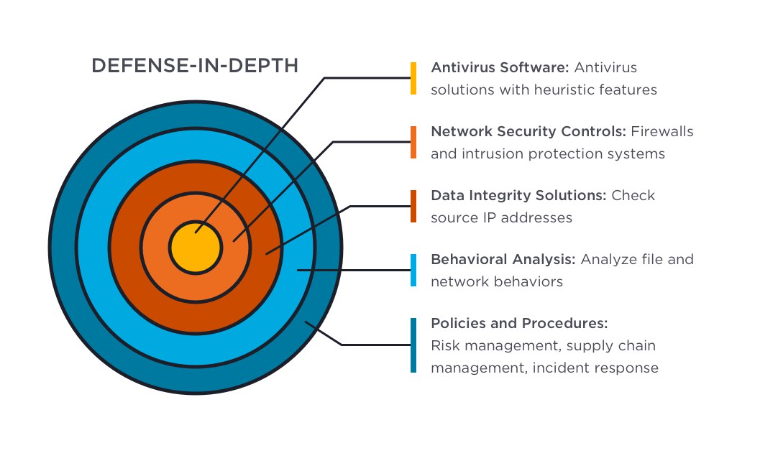
\includegraphics[width=0.8\textwidth]{PhotoMemoire/dep_image.png}
\caption{Un Schéma Illustrant Le DEP \cite{15} }
\end{center}
	\end{figure}
	
	
	
	\pagebreak
	\newpage
	\subsection{Comment mettre en œuvre laec déen pro cybersécurité}
 Le panorama des cybermenaces est en constante évolution. La mise en œuvre d’un solide dispositif de cybersécurité peut donc s’avérer être un véritable défi. Elle n’est toutefois pas impossible,\\
  si les entreprises suivent une approche systématique en intégrant les éléments suivants :
  
  \textbf{Analyse et gestion des risques.} Une approche basée sur les risques garantit que les équipes de sécurité auront connaissance des risques les plus critiques pour l’entreprise, et pourront adopter l’intervention adéquate pour réduire leur impact éventuel.\\
  \textbf{Inventaire et gestion des ressources.} Il est essentiel de comprendre les ressources d’une entreprise pour appréhender et gérer les risques qui menacent ces ressources.
  Identification et gestion des vulnérabilités.\\ Les vulnérabilités doivent être identifiées et corrigées dès que possible, en particulier si elles sont critiques et peuvent véritablement nuire à l’entreprise.\\
  
  \textbf{Déploiement de la gestion des accès et identités.} Pour éviter à la fois les attaques de l’intérieur et de l’extérieur, il est essentiel de protéger et de contrôler l’accès aux services, aux systèmes et aux données.
  
  \textbf{Sécurité des données.} L’ensemble des données organisationnelles doit être protégé de tout accès ou utilisation non autorisés.\\
  
  \textbf{Gestion des incidents.} Une bonne gestion des incidents peut réduire l’impact et les dommages causés par les incidents de sécurité.\\
  
  \textbf{Sécurité de la chaîne logistique.} Il est essentiel d’identifier et d’appréhender de manière cohérente les risques et vulnérabilités sur les réseaux tiers.\\
  
  \textbf{Formation des salariés.} Selon une étude IBM, l’erreur humaine est responsable de 49 pourcent  des violations. Une autre étude de la Stanford University estime que les erreurs humaines, en particulier celles des salariés, est à l’origine de 88 pourcent des violations. Les salariés utilisent souvent des mots de passe faibles, se font avoir par les e-mails d’hameçonnage, ou n’installent pas les mises à jour de sécurité sur leurs appareils. Il est vital de former le personnel aux bonne habitudes de cybersécurité pour bénéficier d’une solide protection.\\
  \paragraph{ }
  L’identification, l’évaluation et la mesure des risques sont des composantes importantes de la mise en place d’un programme de cybersécurité. Sans ces étapes essentielles, les entreprises ne pourront sans doute pas mettre en œuvre un dispositif solide, ni améliorer leur posture de sécurité.
  \begin{figure}[h]
  	 \begin{center}
  	 		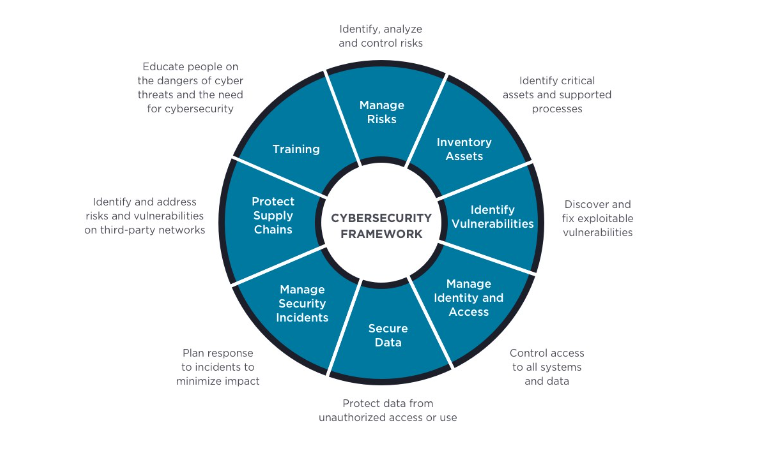
\includegraphics[width=0.8\textwidth]{PhotoMemoire/image_oeuvre.png}
  	 		\caption{Le CyberSecurity Framework \cite{15} }
  	 \end{center}
  \end{figure}
  
 \section{But}
 Le but concret de la cybersécurité est de protéger les systèmes informatiques, les réseaux, les programmes et les données contre les attaques, les dommages, les modifications ou les fuites non autorisées. La cybersécurité vise à prévenir les cyberattaques, à détecter les violations de sécurité, à réduire les dommages potentiels et à réagir efficacement en cas d'incident de sécurité.\\
 \section{objectif}
 L'objectif concret de la cybersécurité est de protéger les systèmes informatiques, les réseaux, les programmes et les données contre les attaques, les dommages, les modifications ou les fuites non autorisées. La cybersécurité vise à prévenir les cyberattaques, à détecter les violations de sécurité, à réduire les dommages potentiels et à réagir efficacement en cas d'incident de sécurité.\\
 \paragraph*{ }
 En 2020, le vol de données et les cyberattaques arrivaient à la 6e et à la 7e place des risques mondiaux les plus importants en termes de probabilité de survenue.\\ En 2021, les hackers continuent d’exploiter la pandémie de COVID-19 et le passage au télétravail opéré en conséquence.\\ Ainsi, les cyberattaques ont augmenté de 21 pourcent dans le monde entier. La cybersécurité joue un rôle crucial pour se tenir à distance de telles menaces et des personnes malveillantes.\\
 
 Les cybercriminels recherchent constamment le talon d’Achille des systèmes informatiques d’entreprise.\\ Pour éviter d’être victimes de cyberattaques, les entreprises doivent mettre en œuvre les outils, les technologies et le personnel adéquats en matière de cybersécurité.\\
\section{La Sécurité Informatique}
\subsection{Définition}
 La sécurité informatique est l'ensemble des mesures techniques, organisationnelles et juridiques mises en place pour protéger les systèmes informatiques, les réseaux et les données contre les attaques, les pertes ou les altérations. Elle vise à garantir la confidentialité, l'intégrité et la disponibilité des informations stockées sur les systèmes informatiques, ainsi que la protection de la vie privée et des droits de propriété intellectuelle. \\

 La sécurité informatique englobe un large éventail de domaines, tels que la sécurité des réseaux, la sécurité des systèmes d'exploitation, la sécurité des applications, la sécurité des données, la sécurité physique, la gestion des identités et des accès, la conformité aux normes de sécurité, la surveillance et la détection des incidents de sécurité, ainsi que la réponse aux incidents de sécurité.\\

  La sécurité informatique est devenue un enjeu majeur dans le monde numérique d’aujourd’hui, où les attaques informatiques sont de plus en plus sophistiquées et fréquentes. La mise en place d'une politique de sécurité informatique efficace est donc essentielle pour protéger les systèmes informatiques et les données sensibles contre les menaces potentielles et assurer la continuité des activités des organisations qui les utilisent.\\
\begin{figure}[h]
	\begin{center}
\includegraphics[width=0.5\textwidth]{PhotoMemoire/image_sec.png}
\caption{Les Différents Points Englobés par La sécurité Informatique \cite{15}}
	\end{center}
\end{figure}

La sécurité informatique englobe plusieurs domaines d'applications :
\begin{enumerate}
\item  sécurité physique et environnementale ;
\item  sécurité de l’exploitation ;
\item   sécurité des réseaux ;
\item  sécurité logique, sécurité applicative 
\item   sécurité de l’information ;
\end{enumerate}
Dans Le cas de notre Serveur Web nous allons voir quels sont les impacts que les différents domaines d'application ont. \\ 
\section*{Sécurité physique et environnementale }
La sécurité physique est souvent définie comme la protection du personnel, du matériel, des logiciels, des réseaux et des données contre les actions physiques et les événements qui pourraient causer des pertes ou des dommages graves à une organisation.\\
La sécurité physique est une pratique commerciale d'une importance vitale avec de nombreux objectifs : empêcher les personnes non autorisées d'entrer dans une entreprise et de causer des dommages ; protéger la propriété intellectuelle contre l'espionnage des entreprises ; et atténuer la violence sur le lieu de travail, entre autres préoccupations.\\
 Aujourd'hui, les organisations doivent considérer la sécurité physique comme un pilier principal de leur stratégie de cybersécurité.\\
 Le succès du programme de sécurité physique d'une organisation peut souvent être attribué à la façon dont chaque composante est mise en œuvre, améliorée et maintenue.\\

\section*{Sécurité de L'information} 
 La sécurité de l'information (infosécurité, infosec) est un ensemble de stratégies de gestion des processus et politiques visant à protéger, détecter, recenser et contrer les menaces ciblant les informations numériques ou non.\\
 Parmi ses responsabilités, l'infosécurité doit établir un ensemble de processus d'entreprise qui protègeront les actifs informationnels indépendamment du format ou de l'état des informations (en transit, en cours de traitement ou stockées au repos).\\
 
 \section*{Sécurité Logique et Applicative}
 La sécurité logique complète la sécurité physique. Sa fonction est de protéger les systèmes, processus et programmes de protection des logiciels et des données, ainsi que l’accès ordonné et autorisé des utilisateurs aux informations.\\
  La sécurité logique comprend toutes les mesures établies par la direction pour minimiser les risques de sécurité associés aux opérations quotidiennes effectuées à l’aide des technologies de l’information, comme le vol d’information, la perte de données, l’entrée de virus, la modification non autorisée de données, les attaques de réseaux, etc.\\
   La sécurité logique vise à préserver la confidentialité, l’intégrité, l’authenticité et la disponibilité des données.\\
 
 La sécurité applicative quant a elle  concerne la manière dont les applications sont développées pour garantir qu'elles sont sécurisées. Elle comprend des mesures de sécurité telles que la validation des entrées, la gestion des erreurs, la gestion des sessions, la gestion des cookies, la protection contre les injections SQL, la protection contre les attaques de script et la protection contre les attaques de force brute. La sécurité applicative vise également à garantir que les applications sont développées selon des normes de sécurité élevées afin de prévenir les vulnérabilités et les failles de sécurité.\\
 
 L’ère numérique a forcé les entreprises à accorder plus d’attention à leur bien le plus précieux: l’information. Aujourd'hui, investir dans la sécurité informatique est vital pour la protection des données de toute organisation. Si vous souhaitez sécuriser vos informations et les protéger contre les attaques, demandez conseil à des experts professionnels en sécurité informatique.
 
 \section*{Sécurité Des Réseau}
 Dans l'infrastructure informatique moderne de l'entreprise, les données sont autant susceptibles d'être en mouvement qu'au repos.\\
  C'est là qu'intervient la sécurité réseau. Si elle fait techniquement partie de la cybersécurité, la sécurité réseau concerne surtout l'infrastructure réseau de l'entreprise.\\
   Elle gère différents aspects notamment la sécurisation de la périphérie du réseau ; les mécanismes de transport des données (commutateurs, routeurs) ; et les dispositifs technologiques qui protègent les données à mesure qu'elles progressent d'un nœud à l'autre.\\
    La principale différence entre cybersécurité et sécurité réseau tient à la mise en œuvre de la planification de la sécurité.\\
    Un plan de cybersécurité sans plan de sécurité réseau est incomplet ; mais un plan de sécurité réseau se suffit à lui-même.\\
 
 \section*{Sécurité de l'exploitation}
 
 L’objectif de la sécurité liée à l’exploitation est de s’assurer que le traitement de l’information est fait de façon correcte et sécurisé. Pour cela, il convient de créer, documenter et diffuser des procédures d’exploitations.
 
 Il est nécessaire de séparer les environnements de tests et d’exploitations afin de réduire les risques sur ce dernier.
 
 \paragraph{La sécurité de l’exploitation c’est aussi :\\}
 \textbf{Un SOC (Security Opérations Center).} Véritable tour de contrôle de la sécurite, le SOC centralise,analyse et répond aux incidents.\\
 
 \textbf{Un SIEM (Security Information and Event Manager).} Le SIEM collecte des informations de l’infrastructure, des systèmes, des applications afin de détecter les attaques.\\
 
\textbf{Le Threat Intelligence ou Cyber Threat Intelligence (CTI)}, est une sorte de profilage de la menace et de l’attaquant permettant une anticipation des attaques.\\
 
 \textbf{Un Tableau de bord (Dashboard)} participe à couvrir les éléments de base de la sécurité à partir d’informations collectées par les équipements de sécurité.\\
 
\textbf{La réponse à incident.} Une fois l’incident survenu il convient de pouvoir y répondre suivant une stratégie établie en amont.\\
 
 \textbf{L’Analyse Forensique} exploite les traces laissées lors d’une attaque afin de connaitre le mode opératoire et éventuellement les utiliser en justice.\\
 
\textbf{La surveillance continue ou ISCM (Information Security Continuous Monitoring)}.
 Elle s’appuie sur d’autres outils comme un SIEM ou un gestionnaire de journaux d’événements. Le but est d’évaluer le niveau de sécurité de l’entreprise et l’évolution du risque en temps réel.\\
 
 \section{La sécurité informatique, pour quoi faire ?}
 La dernière décennie a été marquée par la migration de pratiquement tous les aspects des activités d’une entreprise vers un environnement en ligne. Dès lors, chaque entreprise se retrouve exposée à un risque de cyberattaque, dont le but peut être de voler des informations sensibles, telles que des données clients et des détails de paiement, des éléments de propriété intellectuelle et des secrets commerciaux, ou tout simplement de porter atteinte à la réputation de l’entreprise.\pagebreak

 Par ailleurs, la généralisation du télétravail, la migration vers le cloud et la prolifération des appareils connectés offrent aux pirates informatiques et autres cybercriminels des possibilités quasi infinies d’attaques. Cette surface d’attaque élargie, combinée à la sophistication croissante des cyberadversaires numériques, a imposé aux entreprises de renforcer et d’actualiser leurs pratiques de sécurité afin de protéger leurs ressources basées dans le cloud en particulier.\\
 
 Dans une certaine mesure, la sécurité informatique est une question de droit. En effet, dans certains pays, la loi impose aux entreprises d’investir dans le développement et l’implémentation de concepts de sécurité informatique, tandis que d’autres pays ont fixé des normes strictes en matière de confidentialité et de protection des données.\\
 \section{Types de sécurité informatique}
 \paragraph{ }
 La sécurité informatique est un terme générique qui désigne tout plan, mesure ou outil destiné à protéger les ressources numériques d’une entreprise. La sécurité informatique comprend plusieurs éléments :\\
 
 \textbf{La cybersécurité} a pour but d’assurer la protection des ressources numériques (réseaux, systèmes, ordinateurs, données, etc.) contre les cyberattaques.\\
 
 \textbf{La sécurité des endpoints, ou protection des endpoints,} est l’approche qui vise à protéger les endpoints (ordinateurs de bureau, ordinateurs portables, terminaux mobiles, etc.) contre les activités malveillantes.\\
 
 \textbf{La sécurité du cloud} regroupe la stratégie et les solutions de protection contre les cybermenaces de l’infrastructure cloud, ainsi que de tout service ou application hébergé dans l’environnement cloud.\\
 
 \textbf{La sécurité des applications} couvre toutes les mesures mises en place pour réduire la vulnérabilité des applications et ainsi empêcher tout vol, fuite ou compromission de données ou de code au sein de l’application.\\
 
 \textbf{La sécurité du réseau }désigne les outils, les technologies et les processus utilisés pour protéger le réseau et l’infrastructure critique contre les cyberattaques et les activités malveillantes. Elle inclut un ensemble de mesures préventives et défensives conçues pour refuser tout accès non autorisé aux ressources et aux données.\\
 
 \textbf{La sécurité des conteneurs} est le processus continu de protection des conteneurs, y compris du pipeline des conteneurs, de l’infrastructure de déploiement et de la supply chain, contre les cybermenaces.\\
 
 \textbf{La sécurité de l’IoT} est une subdivision de la cybersécurité qui couvre la protection, la surveillance et la neutralisation des menaces ciblant l’Internet des objets (IoT) et le réseau de terminaux IoT connectés qui collectent, stockent et partagent des données via Internet.\\
 \section{Sécurité informatique et sécurité des informations, quelle différence ?}
 
 Bien que la sécurité informatique soit parfois confondue avec la sécurité des informations, il s’agit de deux concepts bien distincts. La principale différence réside dans la forme dans laquelle les données sont stockées et, par extension, dans la manière dont elles sont protégées.\\
 
 La sécurité des informations consiste à protéger les données, quelle que soit leur forme. Il peut s’agir de protéger les données stockées par voie électronique, ainsi que de mesures de sécurité physiques telles que le verrouillage des armoires de classeurs ou des clés d’accès aux bureaux.\\
 
 La sécurité informatique concerne quant à elle la protection des données et autres ressources exclusivement sous forme numérique.\\
 \section{Sécurité informatique et cybersécurité, quelle différence ?}
 l importe également de faire la distinction entre sécurité informatique et cybersécurité.\\
 
 La cybersécurité fait référence à la protection de l’entreprise contre tout accès non autorisé et toute attaque malveillante.\\
 
 Par comparaison, la sécurité informatique revêt un caractère plus large. Elle couvre notamment toute fonctionnalité permettant de protéger et de préserver la confidentialité, l’intégrité et la disponibilité des données contre toute menace numérique.\\ Cela peut notamment inclure la protection contre les problèmes de sécurité non malveillants en soi, comme un composant matériel défaillant ou une configuration incorrecte du système.\\
 \section{Risques associés à la sécurité informatique}
 Les risques associés à la sécurité informatique peuvent être divisés en deux catégories : les perturbations du système et les attaques malveillantes ciblées.\\
 
 Une perturbation du système peut consister en une interruption temporaire des activités de l’entreprise induite par un composant système tel qu’un composant matériel défectueux, une panne réseau ou une faille logicielle. Face à une telle situation, l’entreprise s’expose à des pertes de revenus résultant de son incapacité à fonctionner ou de l’atteinte possible à sa réputation.\\
 
 Si la préservation du fonctionnement du système constitue une composante majeure de la sécurité informatique, la protection contre les cyberattaques est plus importante encore dans la mesure où la plupart de ces attaques visent à accéder à des données ou autres informations sensibles ou à les dérober. Voici quelques cyberattaques courantes dans Les 2 Tableaux Ci-après :
 
 
    \textbf{Tableau De Cyber Attaques}
   \begin{table}[h]
 		\begin{center}
 		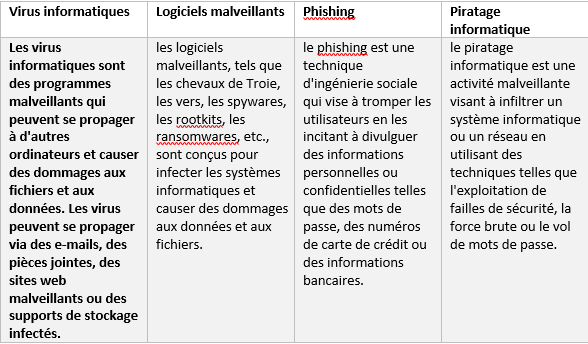
\includegraphics[width=0.7\textwidth]{PhotoMemoire/tableau1_attaques.png}
 		\caption{Tableau 1  Des Attaques}
 		  \end{center}
  \end{table}
 \vspace{2 cm}
 	\begin{table}[h]
 		\begin{center}
 		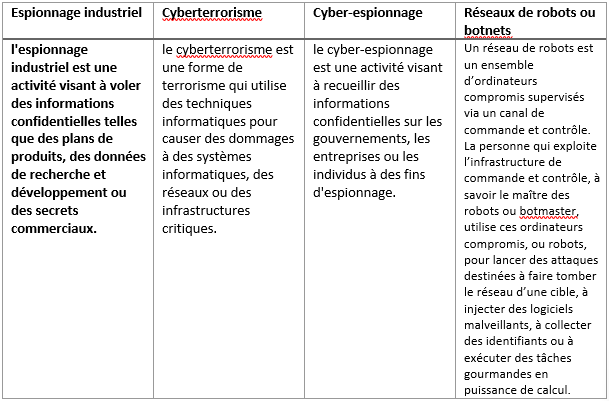
\includegraphics[width=0.7\textwidth]{PhotoMemoire/tableau2_attaques.png}
 		\caption{Tableau 2  Des Attaques}
 		 \end{center}
 	\end{table}
 
\section*{\textbf{Une stratégie de sécurité IT doit intégrer les éléments suivants :}}

\begin{itemize}
	\item[$\bullet$]\textbf{La détection et l’intervention sur les endpoints (EDR)} forment une solution complète qui identifie et contextualise toute activité malveillante afin d’aider l’équipe de sécurité à prioriser les efforts de réponse et de correction en cas de compromission de sécurité.\\
	
	\item[$\bullet$]\textbf{La détection et l’intervention managées (MDR)} sont un service de cybersécurité qui allie technologie et expertise humaine pour mettre en place des opérations de Threat Hunting, de surveillance et d’intervention. La MDR a pour principal avantage de favoriser une identification rapide des cybermenaces et d’en limiter les répercussions sans avoir à augmenter les effectifs.\\
	
	\item[$\bullet$]\textbf{La réponse à incident} consiste en une série d’étapes mises en place pour prévenir, détecter et bloquer les compromissions de données, ainsi que pour restaurer les systèmes. Elle aboutit généralement à l’établissement d’un plan de réponse à incident qui décrit les étapes et procédures que l’organisation devra suivre en cas d’incident de sécurité.\\
	
	\item[$\bullet$]\textbf{Un antivirus de nouvelle génération (NGAV, Next-Generation Antivirus)} combine intelligence artificielle, détection des comportements, algorithmes de Machine Learning et atténuation des exploits, afin d’anticiper et de prévenir immédiatement toutes les menaces de sécurité, connues comme inconnues.\\
	
	\item[$\bullet$]\textbf{Un test d’intrusion} consiste en une simulation d’attaque réelle visant à tester les capacités de détection et de réponse de l’entreprise.
	
   
\end{itemize}
\section*{Qu’attendre d’une antivirus de nouvelle génération ?}


Un antivirus de nouvelle génération efficace doit s’appuyer sur des technologies innovantes pour faire face à des cyberadversaires qui changent constamment de tactiques, techniques et procédures pour s’infiltrer dans les entreprises, qu’il s’agisse de malwares de base ou zero day, ou encore d’attaques avancées sans logiciels malveillants.\\
 Les fonctionnalités de prévention à privilégier sont les suivantes :

\begin{figure}[h]
	\begin{center}
	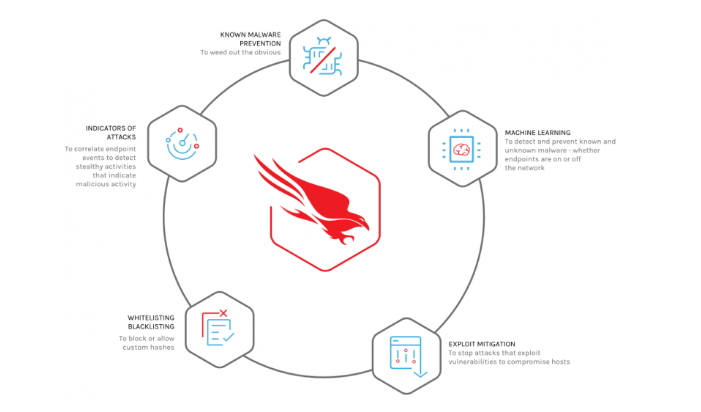
\includegraphics[width=0.9\textwidth]{PhotoMemoire/newgenerationanti.png}
	\caption{Les Différentes Parties Des Antivirus de Nouvelle Génération\cite{15} }
	\end{center}
\end{figure}

\begin{enumerate}
 

 \item  Prévention des logiciels malveillants connus et inconnus
\subitem{a)} Protection antimalware sans fichiers de signatures
 La protection antimalware sans fichiers de signatures utilise des algorithmes de Machine Learning pour déterminer la probabilité qu’un fichier soit malveillant. Les nouvelles menaces sont bloquées en temps réel et la rentabilité est immédiate.
 
 \subitem{b)} Machine Learning
 Le Machine Learning peut détecter et contrer les logiciels malveillants connus et inconnus, que les endpoints soient connectés au réseau ou non. Il détecte les indicateurs d’attaque de manière plus rapide et précise, élimine les ransomwares et comble les failles laissées par les antivirus d’ancienne génération.
 
\item  Prévention des attaques sans logiciels malveillants
 \subitem{a)}. Indicateurs d’attaque
 Les indicateurs d’attaque mettent en corrélation les événements se produisant au niveau des endpoints afin de détecter les activités furtives, signes d’intentions malveillantes.\\ 
 Une solution s’appuyant sur une analyse hors ligne rétrospective pour identifier les indicateurs d’attaque est incapable de rester au fait des dernières cybermenaces, en plus de nécessiter des ressources considérables.\\
  Les algorithmes en ligne qui exploitent le Machine Learning et n’ont pas besoin d’un ensemble complet de données pour effectuer des analyses pertinentes sont à la fois plus rapides, plus efficaces et plus performants.\\
 
 \subitem{b)} Blocage des exploits
 Les malwares ne sont pas toujours distribués au moyen de fichiers. Les attaques basées sur des macros, des commandes d’exécution, des chargeurs en mémoire et d’autres techniques sans fichiers sont en effet de plus en plus courantes.\\
  Le blocage des exploits permet de détecter et de bloquer les exploits dès qu’ils se produisent.\\
 
 \item Intégration de la cyberveille
 L’intégration de la cyberveille permet de déterminer immédiatement l’origine, l’impact et la gravité des attaques dans l’environnement et apporte les conseils nécessaires pour une intervention décisive et une résolution rapide.\\
 
 \item Solution native au cloud
 L’architecture cloud est une composante fondamentale des antivirus de nouvelle génération.\\
  Un NGAV basé dans le cloud peut être totalement opérationnel en quelques secondes, et ce sans redémarrage, mise à jour des signatures, configuration ni acquisition d’une nouvelle infrastructure.\\
   Les algorithmes peuvent traiter en direct l’activité des endpoints et exposer les fichiers malveillants et les comportements suspects en temps quasi réel, sans incidence sur les performances des endpoints.\\
\end{enumerate}

\section{Bonnes pratiques en matière de sécurité informatique}

La prévalence du terme « \textbf{sécurité informatique} » ne signifie nullement que la sécurité est un « \textbf{problème informatique }». Ce n’est pas non plus un problème qui sera résolu uniquement à l’aide de solutions technologiques.\\ Pour élaborer une stratégie de cybersécurité à la fois complète et efficace, les entreprises doivent tenir compte des règles, des processus et des technologies mis en œuvre dans l’ensemble des fonctions métier.\\ Par ailleurs, les utilisateurs du réseau doivent être correctement formés aux comportements responsables en ligne, ainsi qu’à la détection des signes d’attaques réseau courantes.\\
Dans le monde connecté actuel, une stratégie de cybersécurité globale est absolument essentielle. Les stratégies de cybersécurité les plus efficaces combinent ressources humaines et solutions technologiques avancées, telles que l’intelligence artificielle (IA), le Machine Learning (ML) et d’autres formes d’automatisation intelligente, afin d’améliorer la détection des activités anormales et de réduire le délai d’intervention et de correction.\\




\chapter{La Configuration Du Serveur Web (Apache) Et La Sécurisation de ce dernier}

\begin{figure}[h]
    \begin{center}
 
\includegraphics[width=0.4\textwidth]{PhotoMemoire/Xampp.png}
 \caption{Logo De Xampp \cite{18}}
    \end{center}
\end{figure}
Pour La configuration J'ai utiliser le programme XAMPP qui  est un ensemble de logiciels libres qui permet de mettre en place un serveur web local sur votre ordinateur pour tester et développer des applications web. Le nom XAMPP est un acronyme qui représente les logiciels inclus dans l'ensemble :
\begin{enumerate}
	\item  X : toutes les plateformes (Windows, Linux, Mac OS X).
	\item  Apache : serveur HTTP open source.
	\item  MySQL : système de gestion de base de données relationnelle.
	\item  PHP : langage de script côté serveur pour les applications web.
	\item  Perl : langage de script polyvalent.
\begin{figure}[h]
	\begin{center}
			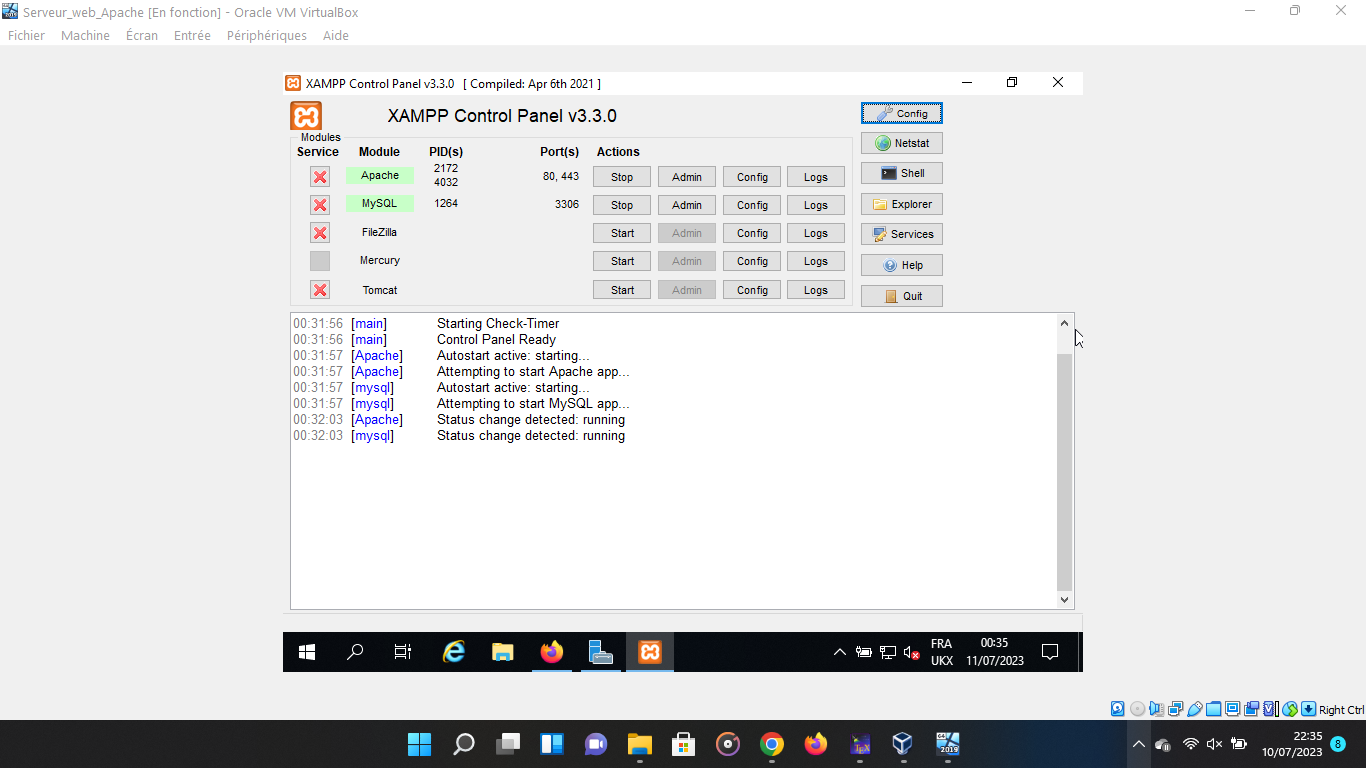
\includegraphics[width=0.7\textwidth]{ PhotoMemoire/Contro Panel.png}
			\caption{Panneau de Configuration et D'administration de Xampp}
	\end{center}
	\end{figure}
\end{enumerate}
XAMPP fournit également des fonctionnalités telles que le support SSL, le support de PHPMyAdmin pour la gestion de bases de données MySQL, et d'autres outils utiles pour le développement et le test d'applications web.\\

L'un des avantages de XAMPP est sa facilité d'utilisation, ce qui le rend particulièrement utile pour les développeurs débutants. XAMPP est disponible gratuitement en téléchargement sur le site Web d'Apache Friends, l'organisation qui développe et maintient XAMPP.


\begin{figure}[h]
	\subsection{Presentaion de Pfsense}
	 \begin{center}
	  	
\includegraphics[width=0.5\textwidth]{PhotoMemoire/pfsense.png}
	  \caption{Logo De Pfsense \cite{18}}
	 \end{center}
	 pfSense est un système d'exploitation open source basé sur FreeBSD qui est utilisé pour construire des routeurs et des pare-feux. Il est conçu pour être facile à installer, à configurer et à administrer, même pour les personnes qui n'ont pas beaucoup d'expérience dans ce domaine.\\
	 
	 pfSense est largement utilisé dans les entreprises, les établissements scolaires, les organisations gouvernementales et les fournisseurs de services Internet pour fournir une connectivité réseau sécurisée et fiable. Il offre des fonctionnalités avancées telles que la gestion de la bande passante, la surveillance de l'utilisation du réseau, le filtrage du trafic, la prise en charge du VPN, la redondance des liens WAN, la haute disponibilité, et bien plus encore.\\
	 
	 Une des caractéristiques de pfSense est la disponibilité d'un système de plug-ins et de packages tiers qui permettent d'ajouter des fonctionnalités supplémentaires au système. Il existe une grande variété de packages disponibles, allant de la surveillance de la sécurité à la gestion des réseaux sans fil.\\
	 
	 pfSense est utilisé par un grand nombre d'utilisateurs à travers le monde, et est considéré comme l'un des meilleurs systèmes d'exploitation pour les routeurs et les pare-feux. Il est également disponible gratuitement en téléchargement sur le site Web pfSense.org.\\
	 
\end{figure}

\begin{figure}[h]
	\section{Configuration de Pfsense(Snorts)}
	
	\begin{center}
		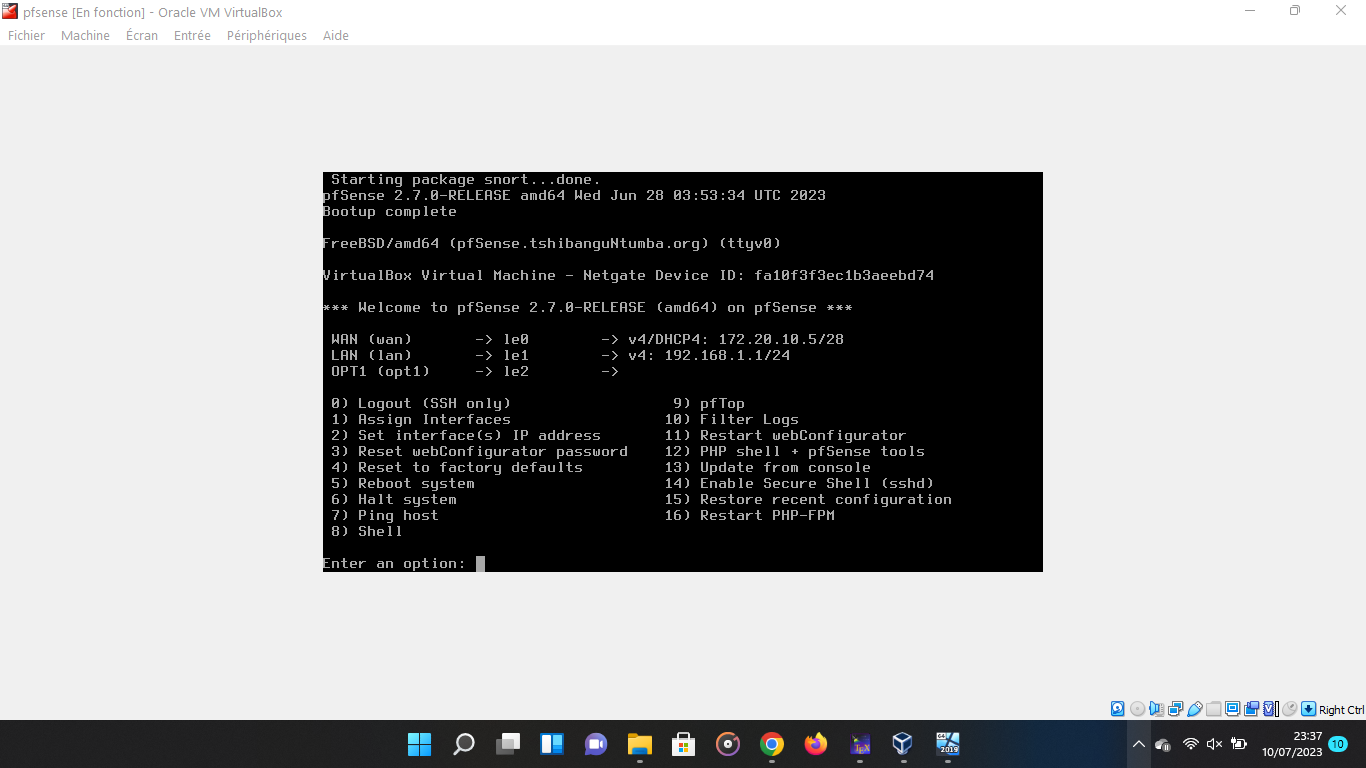
\includegraphics[width=0.8\textwidth]{ PhotoMemoire/interfacepfsense.png}
		\caption{Interface De Pfsense }
	\end{center}
	Sur cette Illustration nous voyons bien que pfsense a deux interface celle qui lui est propre et celle du serveur qu'il protege .
\end{figure}


	  \begin{figure}[h]
	  	\subsection{Configuration du Snort Pfsense} 
	  	\begin{center}
	  		
	  	 	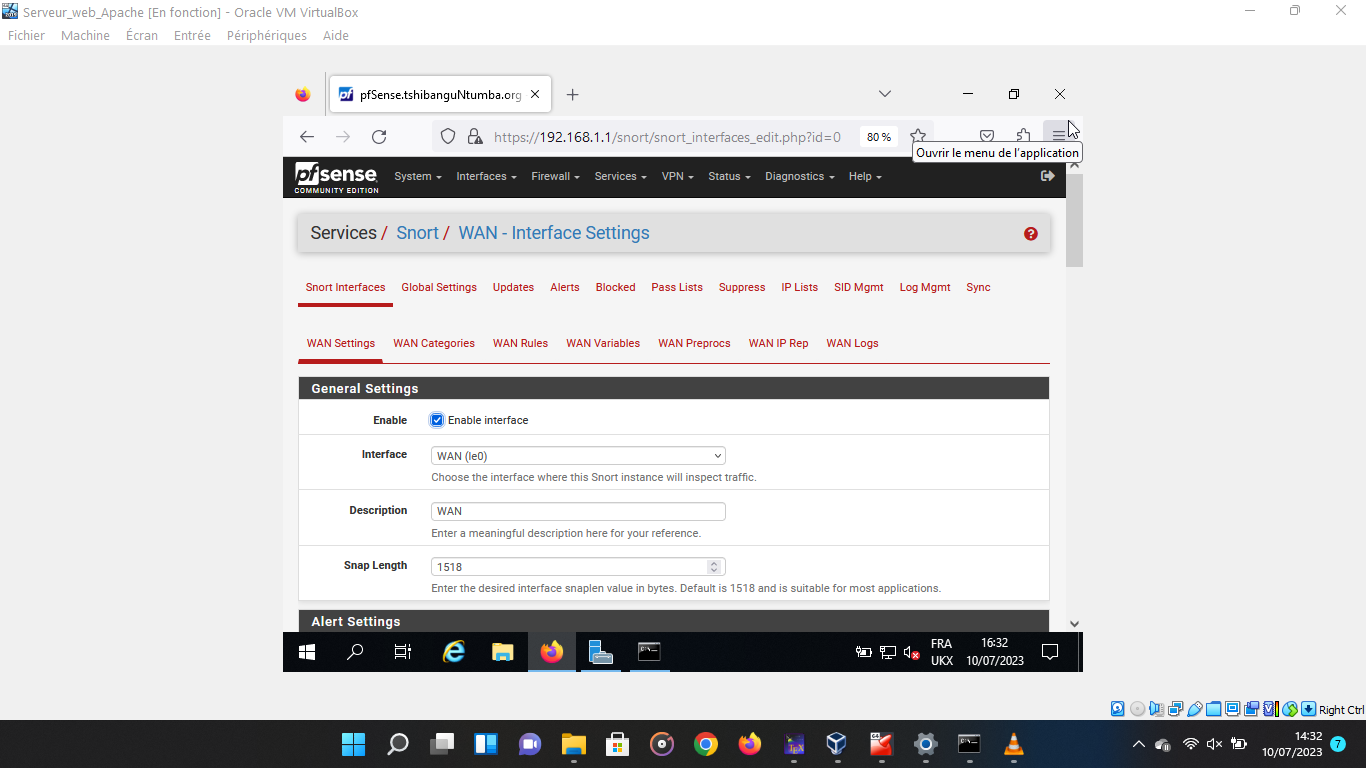
\includegraphics[width=0.8\textwidth]{photo_memoireConfig/configurationInterfaceServeur.png}
	  	 \caption{Interface Web Pfsense }
	  	\end{center}
	 \end{figure}
	 
	 \begin{figure}[h]
	  \begin{center}
	   	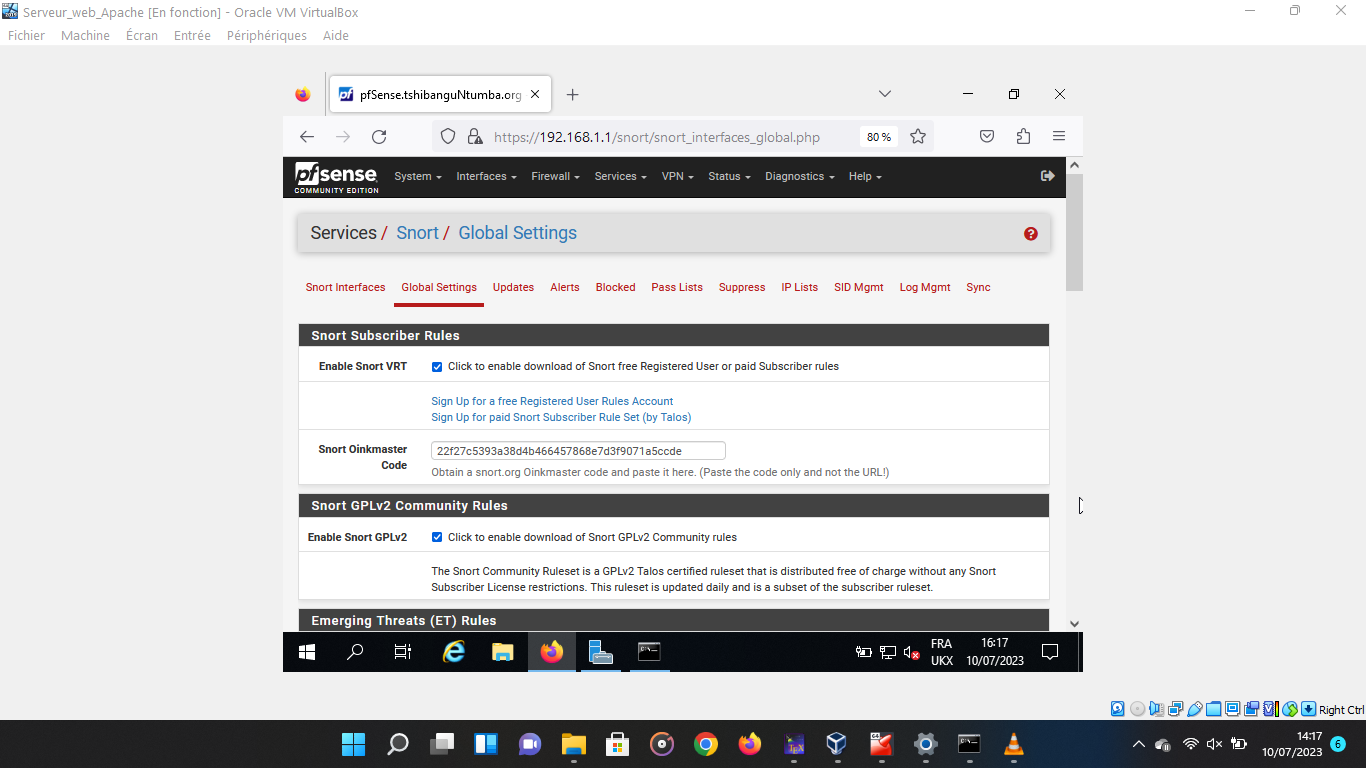
\includegraphics[width=0.8\textwidth]{photo_memoireConfig/Global_settings.png}
	   \caption{Configuration des paramètres Globaux de l'interface}
	    \end{center}
	 \end{figure}
	 
	 \begin{figure}[h]
	 	  \begin{center}
	 	 	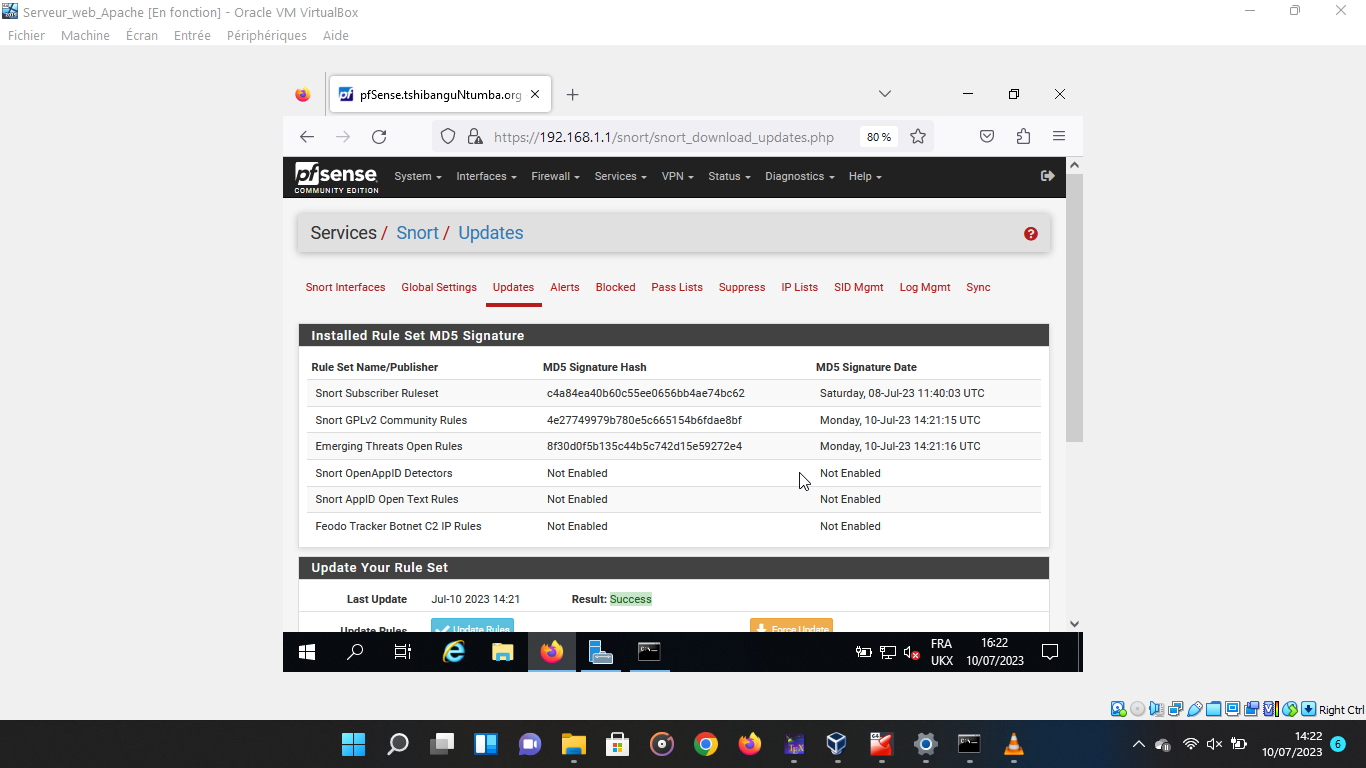
\includegraphics[width=0.8\textwidth]{photo_memoireConfig/Update_des Cles MD5.png}
	 	 \caption{Mise  a jour des clés de chiffrements MD5, Et des Règles de Filtrage }
	\end{center}
	 \end{figure}
 


\begin{figure}[h]
	\section{Capture Des Test}
	\paragraph{}
	Ici nous voyons clairement que le Snort a Bel et bien intercepter l'adresse IP
	De l'attaquant  et alerte L'interface Web d'une tentative d'intrusion.
 \begin{center}
			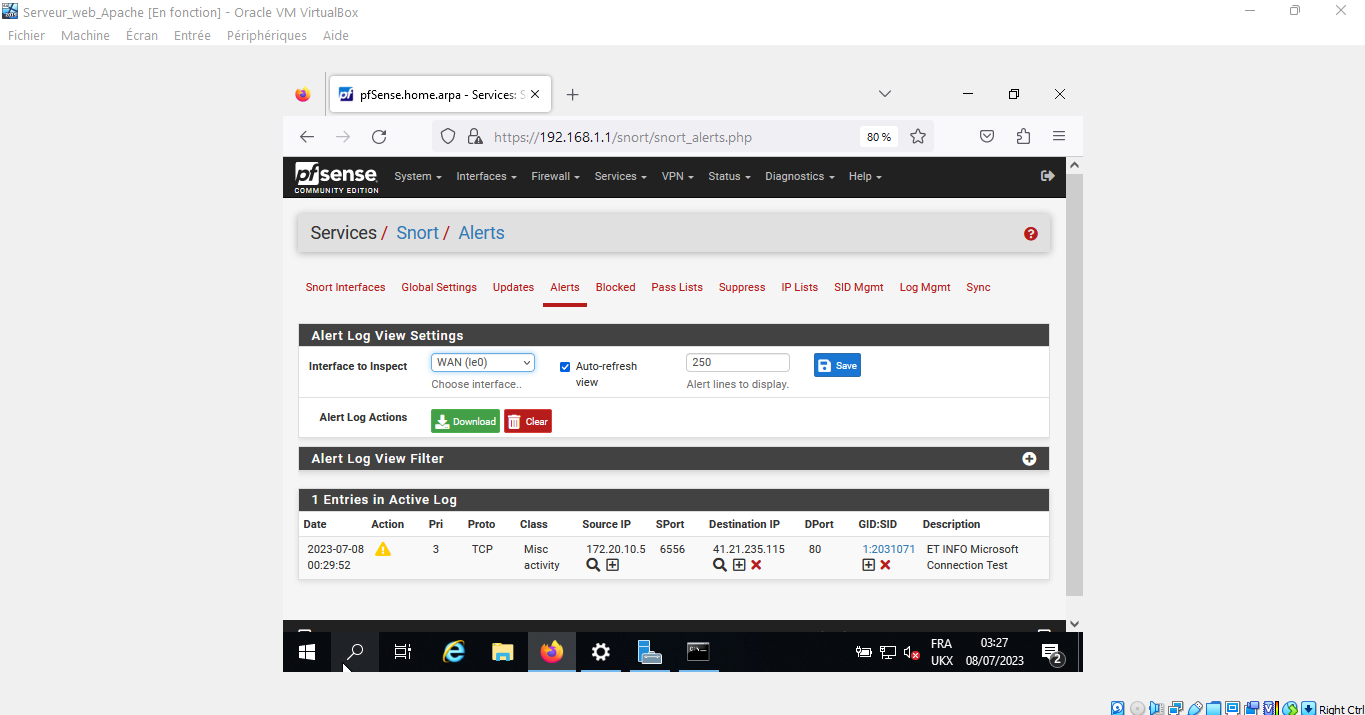
\includegraphics[width=0.8\textwidth]{photo_memoireConfig/Alert_ip.png}
		\caption{Alerte D'intrusion Pfsense}
	\end{center}
\end{figure}
 
\begin{figure}[h]
	\paragraph{}
	Sur cette Illustration on voit que le Snort a bloquer l'adresse de l'attaquant et l'a interdit d'accès.
	 \begin{center}
		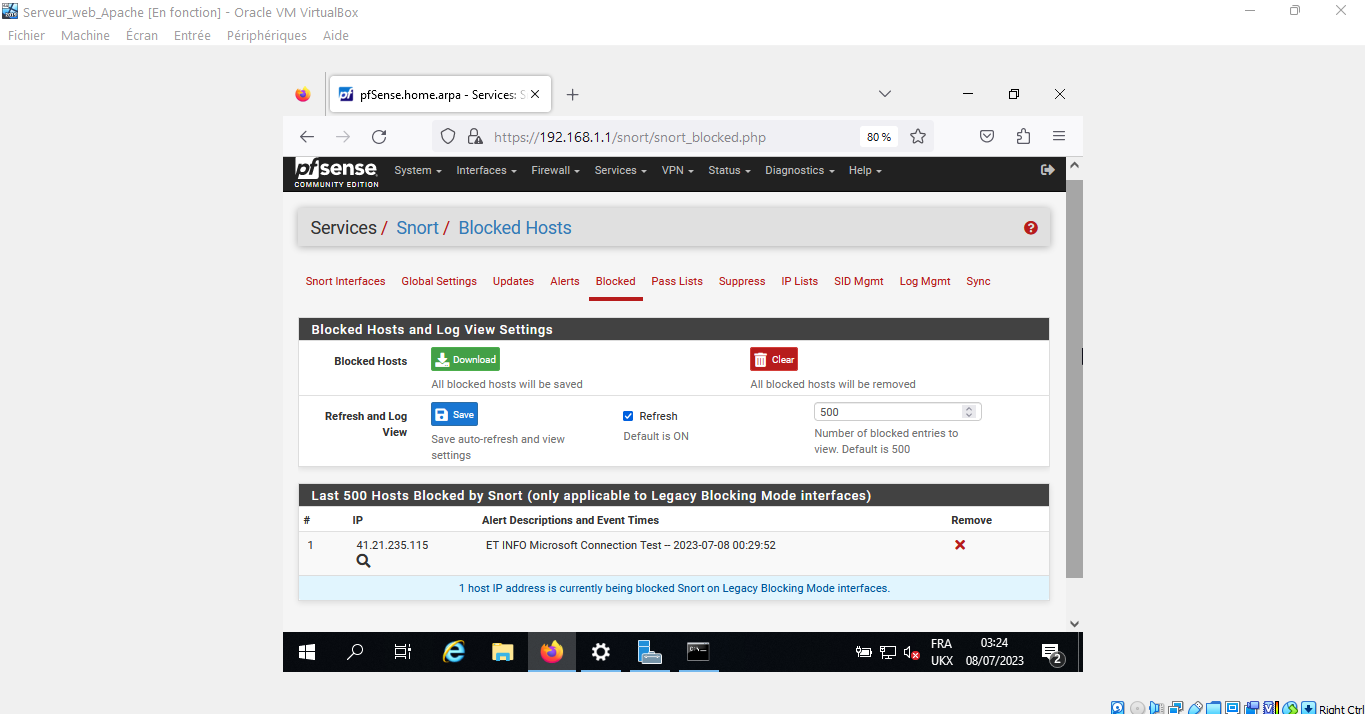
\includegraphics[width=0.8\textwidth]{photo_memoireConfig/Blocked_IP.png}
		\caption{Adresse Ip Isolées}
 \end{center}
\end{figure}
 
\begin{figure}[h]
	\section{Environnement de Test}
	\subsection{Virtual Box}
	\begin{center}
		
\includegraphics[width=0.8\textwidth]{PhotoMemoire/Virtualbox.png}
		\caption{ Le logo Virutal Box }\cite{18}
	\end{center}
	Oracle VirtualBox est un logiciel de virtualisation open source qui permet de créer des machines virtuelles sur votre ordinateur. Les machines virtuelles sont des environnements virtuels qui peuvent exécuter différents systèmes d'exploitation, tels que Windows, Linux, MacOS et bien d'autres, à l'intérieur d'un hôte (votre ordinateur).\\
	
	VirtualBox est utilisé pour de nombreuses tâches, notamment pour tester des applications, pour développer des logiciels, pour créer des environnements de test, pour exécuter des systèmes d'exploitation différents, pour configurer des serveurs en environnement isolé, etc.\\
	
	VirtualBox fonctionne en émulant des composants matériels tels que le processeur, la mémoire, le stockage et les interfaces réseau. Il fournit également des fonctionnalités avancées telles que le partage de fichiers entre l'hôte et la machine virtuelle, la prise en charge de l'USB, la virtualisation des cartes graphiques, la prise en charge de plusieurs écrans, et bien plus encore.\\
	
	VirtualBox est développé et maintenu par Oracle Corporation et est disponible en téléchargement gratuit sur son site Web. Il est compatible avec une grande variété de systèmes d'exploitation hôtes, notamment Windows, Linux, MacOS et Solaris.\\ 
\end{figure}

\begin{figure}[h]
	Les machines Virtuelle on permis les différents test dans ce Travail.
	 \begin{center}
	 	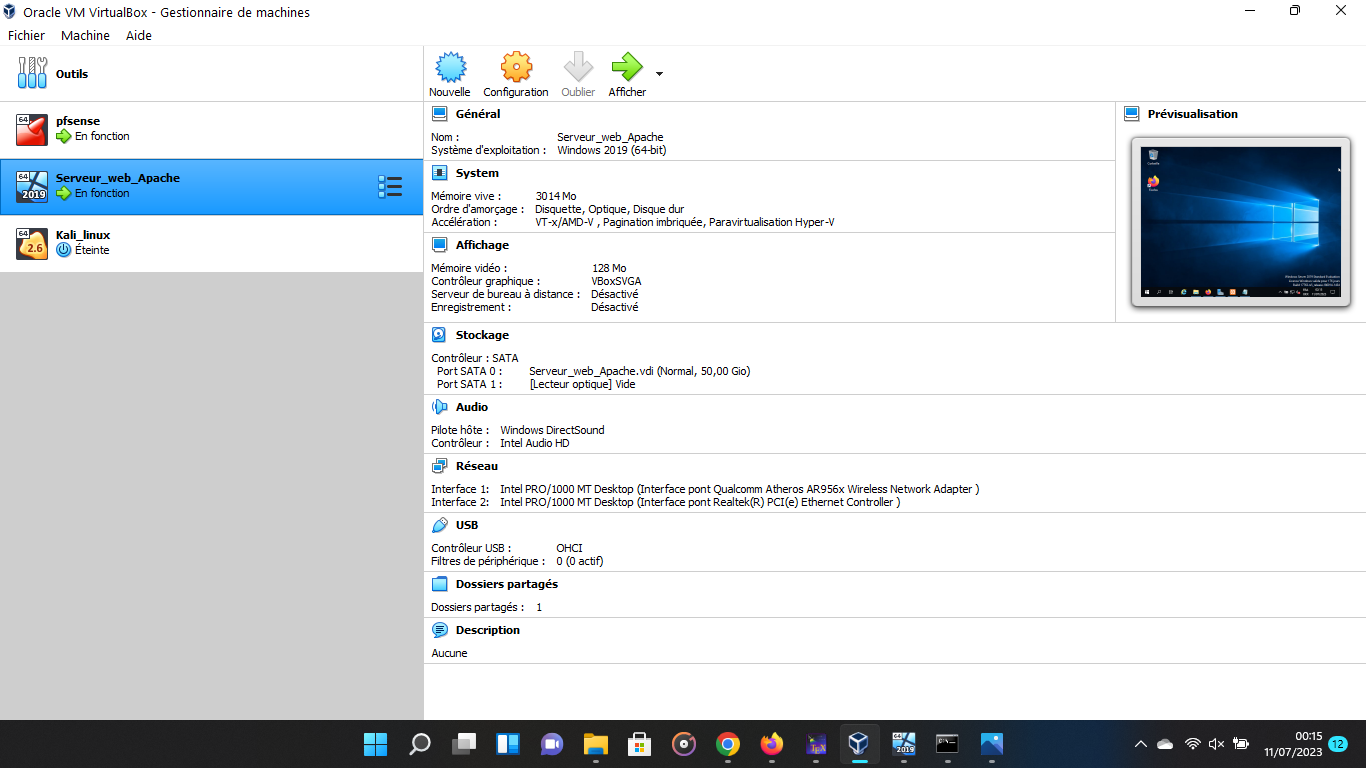
\includegraphics[width=0.8\textwidth]{PhotoMemoire/machineutilisee.png}
	 	\caption{ Les Machines Utilisées Pour les Test}	
	 \end{center}
\end{figure}
\begin{figure}[h]
	 Site Web Utilisé Pour Les Test
	\begin{center}
		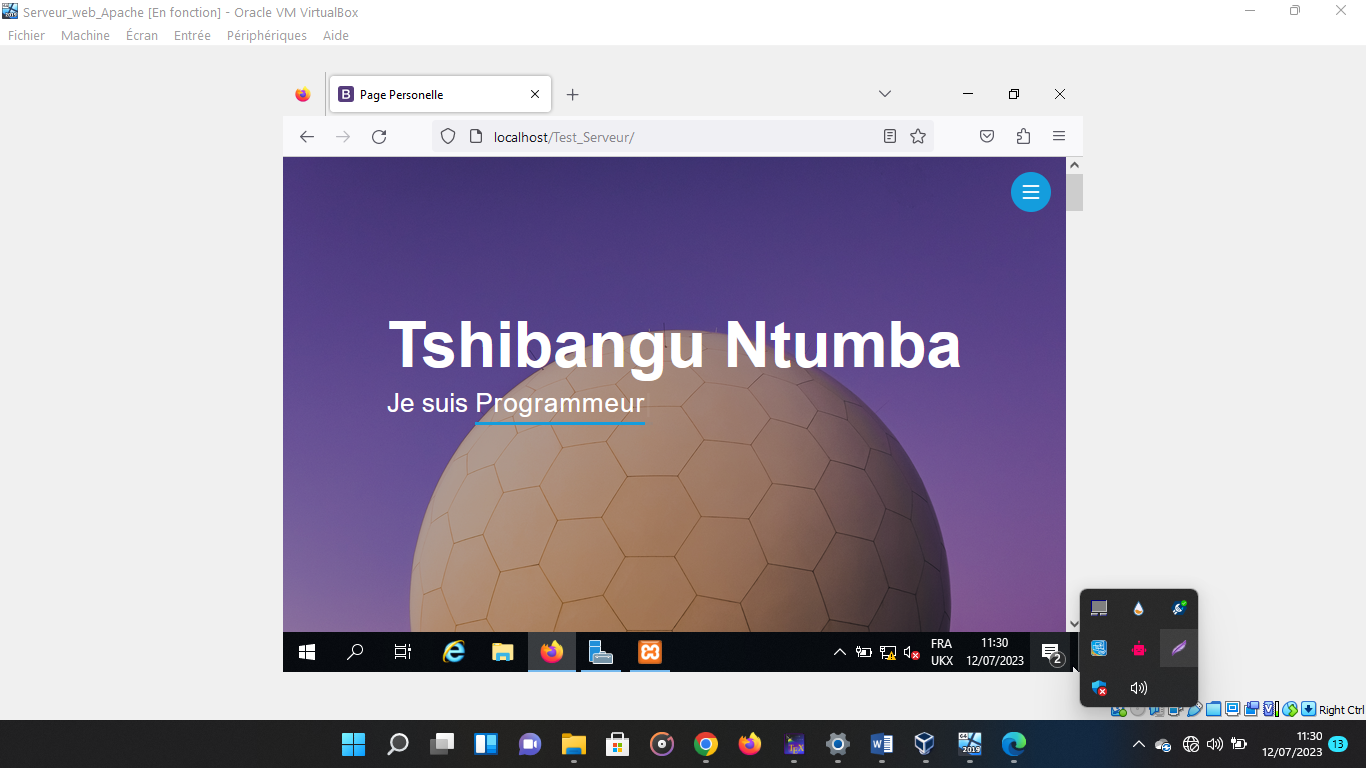
\includegraphics[width=0.8\textwidth]{PhotoMemoire/serveur _Web.png}
		\caption{ Site Web Utilisé Pour les Test}
	\end{center}
\end{figure}





\newpage

\begin{thebibliography}{9}
	\section*{Ouvrages}
	\bibitem{sol19} Solange Ghernaouti,\emph{ Cybersécurité Analyser les risques	Mettre en œuvre	les solutions}.
	Dunod,
	6 ème Ed,
	2019.
	 
	\bibitem{muk} Patrick Mukala, \emph{THEORIE DE L’INFORMATION ET CRYPTOGRAPHIE : Principes 
	Fondamentaux.}\\
	 
     \bibitem{sol19} Solange Ghernaouti,\emph{ Cybersécurité sécurité informatique  et réseaux }.
     Dunod,
     5 ème Ed,
     2011.
      
     \bibitem{Lis19} Lisa Bock, \emph{Learn Wireshark.}
      Packt Publishing
      1 ère Ed,
      2019.
	
	\section*{  Webography \hrule}
	
	\bibitem{1} \href{https://developer.mozilla.org/fr/docs/Learn/Common_questions/Web_mechanics/What_is_a_web_server}{\emph{MDN Web Docs.}} \\
	\bibitem{2}\href{https://www.sartagas.fr/outils-de-la-ssi/securite-de-l-exploitation/}{\emph{Sécurité de l’exploitation – Sartagas votre guide d'outils informatiques pour votre CyberSécurité.}}
	\bibitem{3}\href{https://www.hostinger.fr/tutoriels/serveur-web}{\emph{Hostinger Tutoriels.}}
	\bibitem{4}\href{https://fr.linkedin.com/pulse/7-conseils-pour-am%C3%A9liorer-la-s%C3%A9curit%C3%A9-physique-dans-jo%C3%ABl#:~:text=La%20s%C3%A9curit%C3%A9%20physique%20est%20souvent,dommages%20graves%20%C3%A0%20une%20organisation.}{\emph{7 CONSEILS POUR AMÉLIORER LA SÉCURITÉ PHYSIQUE DANS VOTRE ENTREPRISE.}}
	\bibitem{5}\href{https://www.departement-ti.com/les-aspects-de-securite-dun-centre-de-donnees/}{\emph{Departement-IT}}
	\bibitem{6}\href{https://learn.microsoft.com/fr-fr/microsoft-desktop-optimization-pack/appv-v4/how-to-configure-the-server-for-iis}{Les Serveurs IIS.}
	\bibitem{7}\href{https://www.1min30.com/dictionnaire-du-web/serveur-web}{\emph{Dico Du Serveur WEB}}
	\bibitem{8}\href{https://www.crowdstrike.fr/cybersecurity-101/it-security/}{\emph{Definition De la CyberSécurité}}
	\newpage
	\section*{Cours Impliqués \hrule}
 
		\bibitem {} Sécurité  informatique.\\
		\bibitem {} Administration Réseaux.\\
		\bibitem {} Introduction Réseau.\\
		\bibitem {} Laboratoire Réseau .\\
		\bibitem {} Architecture des ordinateurs .\\	 
	
	
\end{thebibliography}

\end{document}